\chapter{Learning Prob. Submodular Models} \label{ch:genes}

\section{Introduction}
As discussed at the very beginning of the thesis, learning probabilistic models from data is one of the main motivations of our work
The probabilistic framework we employ suggests a principled way to estimate the model parameters given a data set, namely by maximizing the model likelihood under the data.
Unfortunately, the maximum likelihood problem for the model class we consider is, in general, non-convex; even worse, evaluating the likelihood function or its gradient with respect to the model parameters boils down to computing expectations over the distribution at hand, which we have already seen to be a hard problem.
We show in this chapter how we can use sampling to approximate the likelihood gradient, and, thus, perform an approximate gradient ascent procedure that converges to a local optimum of the model likelihood.
Then, we focus on applying this learning procedure to the application of modeling the interactions between gene mutations in cancer patients.
We evaluate our method on synthetic and real cancer data, visualize the results in several ways, and compare them to the state of the art.


\section{Approximate Maximum Likelihood Learning using Sampling} \label{sect:ml}

As before, we consider a model of the form
\begin{align*}
p(S; \btheta) = \frac{1}{Z(\btheta)} \exp\left( F(S; \btheta) \right),
\end{align*}
parametrized by a vector $\btheta$, which we would like to learn.
Given a data set of $N$ sets, $\mathcal{D} \defeq (D_1,\ldots,D_N)$, $D_1,\ldots,D_N \subseteq V$, the log-likelihood of the model is
\begin{align*}
\ell(\btheta) &\defeq \sum_{i=1}^N \log p(D_i; \btheta)\\
           &= \sum_{i=1}^N \left( F(D_i; \btheta) - \log Z(\btheta) \right)\\
           &= \sum_{i=1}^N F(D_i; \btheta) - N \log Z(\btheta).
\end{align*}
The gradient of the log-likelihood with respect to the parameters $\btheta$ is
\begin{align*}
                 \*g(\btheta) &\defeq \nabla_{\btheta} \ell(\btheta)\\
                              &= \sum_{i=1}^N \nabla_{\btheta} F(D_i; \btheta) - N \nabla_{\btheta} \log Z(\btheta)\\
                              &= \sum_{i=1}^N \nabla_{\btheta} F(D_i; \btheta) - N \frac{1}{Z(\btheta)} \nabla_{\btheta} Z(\btheta)\\
                              &= \sum_{i=1}^N \nabla_{\btheta} F(D_i; \btheta) - N \frac{1}{Z(\btheta)} \nabla_{\btheta} \sum_{S \subseteq V} \exp\left( F(S; \btheta) \right)\\
                              &= \sum_{i=1}^N \nabla_{\btheta} F(D_i; \btheta) - N \sum_{S \subseteq V} \frac{\exp\left( F(S; \btheta)\right)}{Z(\btheta)} \nabla_{\btheta} F(S; \btheta)\\
                              &= \sum_{i=1}^N \nabla_{\btheta} F(D_i; \btheta) - N \sum_{S \subseteq V} p(S; \btheta) \nabla_{\btheta} F(S; \btheta)\\
                              &= \sum_{i=1}^N \nabla_{\btheta} F(D_i; \btheta) - N\,\E_{p}\left[ \nabla_{\btheta} F(S; \btheta) \right]\\
                              &= \frac{1}{N}\sum_{i=1}^N \nabla_{\btheta} F(D_i; \btheta) - \E_{p}\left[ \nabla_{\btheta} F(S; \btheta) \right].
\end{align*}
This shows that the maximum likelihood parameters satisfy a generalized version of the well-known moment matching condition for exponential family models; cf. \cite[Ch. 20]{koller09}.
That is, at the maximum, the empirical mean of the function gradient over the data set will match the expected gradient over the model distribution.

While the expectation term in the log-likelihood gradient is, in general, infeasible to compute exactly, we can straightforwardly approximate it using the sampling methods discussed in the previous chapters.
In particular, if we have drawn samples $\mathcal{S} = \{ S_1,\ldots,S_M \}$, $S_1,\ldots,S_M \subseteq V$, from distribution $p$, we can approximate the gradient $\*g(\btheta)$ by
\begin{align*}
\widetilde{\*g}(\btheta) \defeq \frac{1}{N}\sum_{i=1}^N \nabla_{\btheta} F(D_i; \btheta) - \frac{1}{M}\sum_{i=1}^M \nabla_{\btheta} F(S_i; \btheta).
\end{align*}
We, therefore, propose learning the parameters $\btheta$ using an approximate gradient ascent procedure, which involves alternating between sampling from the current model to compute $\widetilde{\*g}(\btheta)$, and performing a gradient step towards the direction of $\widetilde{\*g}(\btheta)$, as shown in \algoref{alg:grad}.

\begin{algorithm}[tb]
  \setstretch{1.2}
  \caption{Approximate maximum likelihood maximization}
  \label{alg:grad}
    \begin{algorithmic}[1]
      \REQUIRE Data $\mathcal{D}$, iterations $n_{\mathrm{iter}}$, samples $M$, step $(\gamma_i)_i$, gradient oracle $\nabla_{\btheta} F(S; \btheta)$
      \STATE Initialize $\theta$
      \FOR{$i = 1$ \TO $n_{\mathrm{iter}}$}
        \LET{$\mathcal{S}$}{sample $M$ sets from $p(\cdot\,; \theta)$}
        \LET{$\widetilde{\*g}(\btheta)$}{$\frac{1}{N}\sum_{i=1}^N \nabla_{\btheta} F(D_i; \btheta) - \frac{1}{M}\sum_{i=1}^M \nabla_{\btheta} F(S_i; \btheta)$}
        \LET{$\btheta$}{$\btheta + \gamma_i\,\widetilde{\*g}(\btheta)$}
      \ENDFOR
      \RETURN $\btheta$
    \end{algorithmic}
\end{algorithm}

\paragraph{Gradients of the \fldc{} model.}
Since we will be focusing on the \fldc{} model for the remainder of this chapter, we derive here the gradients of its potential function with respect to its parameters.
For simplicity, we assume that we use an equal number of $L$ dimensions for both the repulsive and the attractive matrices.
As a reminder, the \fldc{} model is then defined via the following potential \citep{djolonga16mixed},
\begin{align*}
F(S; \bu, \bw, \bv) = \sum_{i \in S} u_i + \sum_{j=1}^{L} \left(\max_{i \in S} w_{ij} - \sum_{i \in S} w_{ij}\right) - \sum_{j=1}^{L} \left(\max_{i \in S} v_{ij} - \sum_{i \in S} v_{ij}\right).
\end{align*}
$F$ is differentiable almost everywhere, due to the presence of the two ``$\max$'' functions.
For the points where it is not differentiable, we define subgradients that give equal contribution to all elements that belong to the corresponding ``$\argmax$''.
In particular, for all $i \in V$, $j \in [L]$, we have
\begin{align*}
\nabla_{u_i} F(S; \bu, \bw, \bv) &= \ind[i \in S]\\
\nabla_{w_{ij}} F(S; \bu, \bw, \bv) &= \frac{\ind[i \in \argmax_{r \in S} w_{rj}]}{|\argmax_{r \in S} w_{rj}|} - \ind[i \in S]\\
\nabla_{v_{ij}} F(S; \bu, \bw, \bv) &= -\frac{\ind[i \in \argmax_{r \in S} v_{rj}]}{|\argmax_{r \in S} v_{rj}|} + \ind[i \in S].
\end{align*}
\citet{tschiatschek16} used an alternative set of subgradients, involving randomization over the choice of the ``$\argmax$'' at each gradient step.
We have noticed that our choice often results in slightly improved learning performance in practice.


\section{Modeling Gene Interactions in Cancer}
One of the goals of cancer genomics research is identifying so-called driver mutations, that is, somatic mutations that are responsible for various forms of cancer, and distinguishing them from randomly occurring passenger mutations.
While sequencing data from large-scale projects, such as The Cancer Genome Atlas \citep{tcga}, has been available in increasing quantities, analyzing the occurence combinations of mutations is a combinatorially daunting task.

Driver mutations often occur in a limited number of key biological pathways, and it has been observed that multiple mutations involved in the same pathway tend to not occur together in the same patient \citep{yeang08}.
As a result, it is of interest to discover groups of gene alterations that are (approximately) mutually exclusive.
Finding such a group is then be indication that the participating mutations are part of the same cancer-related pathway.
Since most existing pathway databases lack in detail and accuracy, there has been particular interest in \emph{de novo} methods, that is, methods that analyze the existing patient data without using any prior biological knowledge, and try to identify new potentially significant combinations of mutations.
For a general review of the topic, we refer to \cite{raphael14}.

Previous \emph{de novo} methods have used different combinatorial or statistical scores to assess the degree of mutual exclusivity of a group of mutuations.
These are then paired with some discovery algorithm that exhaustively enumerates groups \citep{muex,yeang08}, progressively builds up larger groups from smaller ones \citep{mutex,rme,memo,timex}, or performs a randomized search in the group space \citep{dendrix,multidendrix,comet}.
As a result, these methods either scale poorly in the number of mutations at hand, or require a prior assumption on the exact or maximum size of the groups to be discovered.
In the following sections, we compare our results against the CoMEt algorithm \citep{comet}, which is a state-of-the-art method for discovering multiple groups of mutually exclusive mutations.
While CoMEt requires prespecifying the number and size of groups to be searched for, it is able to produce in the end a consensus of arbitrarily sized groups.

\subsection{Probabilistic Modeling of Gene Mutations}
Assume that we are given a ground set $V = \{1,\ldots,n\}$ of possible gene mutations, and a data set of $N$ patients, $\mathcal{D} \defeq (D_1,\ldots,D_N)$, where $D_i \subseteq V$ is the combination of mutations that were present in patient $i$.
The data is commonly represented in the literature using a binary alteration matrix, as shown in \figref{fig:bamats} (top), where each row represents a mutation, and each column a patient.
Our goal is to discover groups of mutations $M_1, M_2, \ldots$, $M_i \subseteq V$, with the property that mutations that belong to the same group rarely occur together in the same patient.
\figref{fig:bamats} (bottom) depicts a permuted version of the previous matrix, where the highlighted group of four mutations appears to be highly mutually exclusive.

\begin{figure}[htb]
\centering
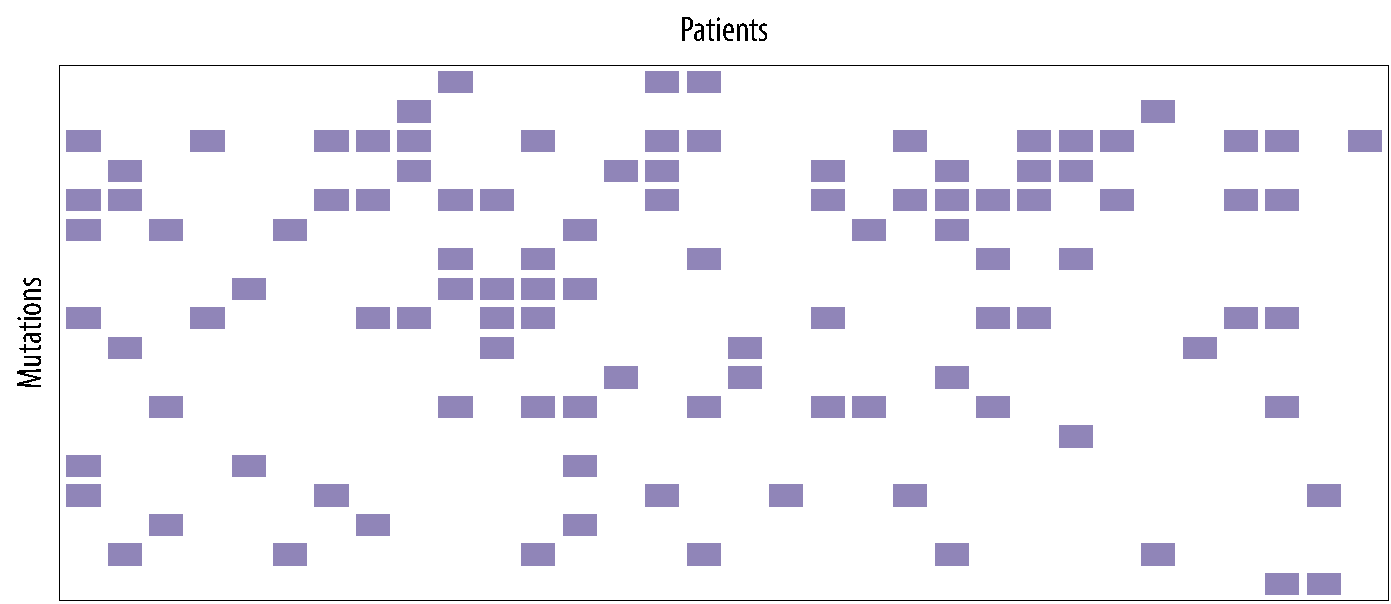
\includegraphics[width=\textwidth]{figures/genes/example1.pdf}\\[1em]
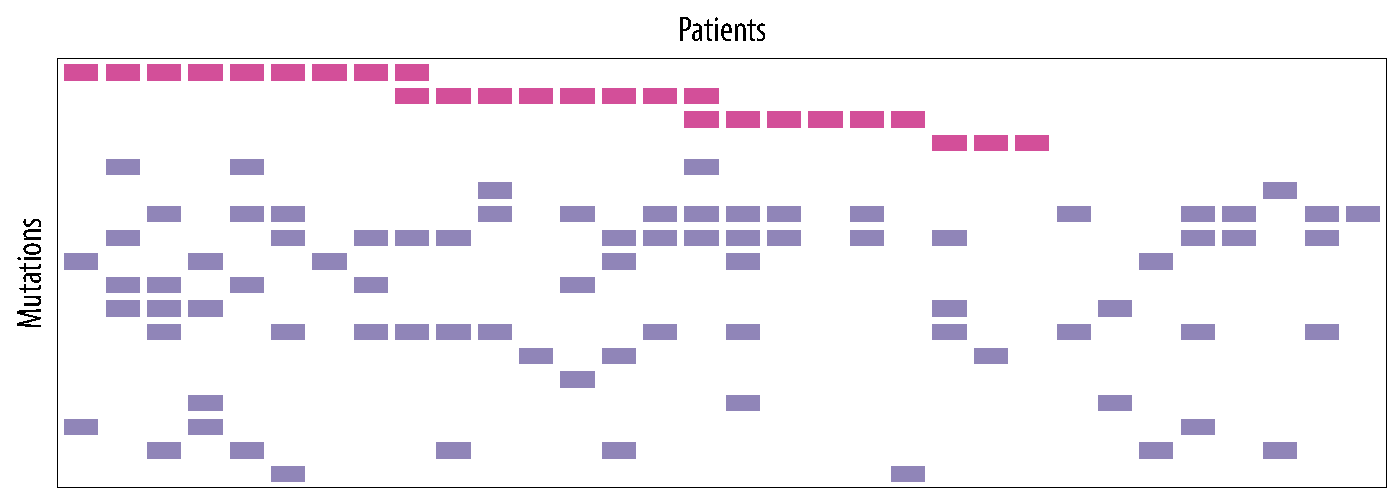
\includegraphics[width=\textwidth]{figures/genes/example1_rep.pdf}\\[1em]
\caption{(top) An example binary alteration matrix, where each shaded entry $(i, j)$ indicates that mutation $i$ occured in patient $j$. (bottom) The same matrix with permuted rows and columns to illustrate the high degree of mutual exclusivity of the highlighted group of four mutations.}
\label{fig:bamats}
\end{figure}

We propose using the patient data $\mathcal{D}$ to learn an \fldc{} model over the mutation space $V$.
Based on the definiton of the \fldc{} potential, we expect the columns of the $\bw$ and $\bv$ matrices to encode groups of repulsive and attractive mutations respectively.
For the purposes of this thesis, we propose extracting potential groups by thesholding each matrix at a specified level; these groups can then be further assessed for mutual exclusivity or co-occurence using some of the previously proposed statistical tests.
More generally, one can perform marginal/conditional inference in the learned model to compute arbitrary probabilistic quantities that may be useful in specific biological applications.

Our approach offers several advantages over previous work.
First, it inherently uses higher-order potentials to directly capture mutation interactions of arbitrary size, without any need to specify the number or sizes of the groups in advance.
Second, in addition to mutual exclusivity, it also models mutation co-occurence, which may also be useful in cancer research \citep{yeang08,raphael14}.
Finally, in terms of computational complexity, the only potentially super-linear component in our learning procedure is the number of samples required to get an accurate gradient approximation.
As we have previously seen, proving general bounds on the mixing time is a hard endeavour, but practical experience shows that our algorithm only takes a few minutes to run on data sets of hundreds of mutations.


\section{Experiments}
In this section, we practically apply our learning algorithm to the problem of modeling gene interactions outlined above.
We begin with providing some more details about each step of the procedure we use to discover mutually exclusive groups of mutations.
The steps for discovering co-occurring groups are analogous.

\paragraph{Step 1: Learning the \fldc{} model.}
We use the approximate maximum likelihood method described in \sectref{sect:ml}.
By definition of the \fldc{} model, the elements of matrices $\bw$ and $\bv$ must be non-negative.
To achieve this during learning, we project the entries of $\bw$ and $\bv$ to the positive orthant after each gradient step.
Furthermore, we have found it beneficial in practice to induce sparsity on these matrices, in order to reduce the effect of noisy data on the learned models, and obtain more interpretable solutions.
To this end, we employ an $L_1$ regularization to both $\bw$ and $\bv$ by projecting each row and column of this matrices to the corresponding $L_1$-ball after each gradient step.

We initialize the entries of $\bu$ to the maximum likelihood estimates of the respective product distribution, that is,
\begin{align*}
u_i = \log\left( \frac{f_i}{1 - f_i} \right),
\end{align*}
where $f_i$ is the frequency of element $i \in V$ in the data set $\mathcal{D}$.
We randomly initialize the entries of $\bw$ and $\bv$ by drawing from a uniform distribution $\mathcal{U}[0, 0.01]$.
To avoid duplicate latent dimensions in the two matrices, for the first half of the iterations, we check the columns of $\bw$ and $\bv$ after each gradient step, and reinitialize a column when we detect that its $L_1$ distance to another column of the same matrix is smaller than a predefined threshold.

Unless otherwise stated, we use $n_{\mathrm{iter}} = 2\cdot10^4$ gradient iterations, and $M = 100|V|$ samples per iteration.
We use the combined sampler detailed in \chapref{ch:m3} with a mix of $100$ random sub- and supergradients, and a combination weight of $\alpha_c = 0.5$.
Finally, we use a fixed step size ($\gamma = 5\cdot10^{-4}$) for the first half of the iterations, and a geometrically decreasing step size ($\gamma_i = \gamma r^i$ with $r = 10^{-3/n_{\mathrm{iter}}}$) for the second half.

\paragraph{Step 2: Extracting proposed mutation sets.}
We start by thresholding each column of the learned $\bw$ matrix at a fixed level $w_{\mathrm{th}} = 1.5$.
We then proceed to create a graph that contains one clique of nodes for each group extracted in the previous step.
Our proposed mutation sets consists of all maximal cliques in this constructed graph.
Creating the graph, rather than directly proposing the groups extracted from the matrix columns, can be useful for merging smaller groups of genes that have been encoded in separate columns of $\bw$ during learning.

\paragraph{Step 3: Testing mutual exclusivity.}
We make use of two statistical tests for testing the degree of mutual exclusivity of a mutation group.

The first was proposed by \cite{mutex}, and used as part of the Mutex algorithm.
For each gene in a proposed mutation group, we run Fisher's one-tailed exact test on the contingency table that results from examining the occurences of that gene in the data set versus the union of all other genes in the group.
This results in one $p$-value per gene in the mutation group, and the output of the test is the maximum of these $p$-values.
We will call this the ``one vs. all'' test, and denote its output $p$-value by $p_{\mathrm{ova}}$.

The second was proposed by \cite{comet}, and used as part of the CoMEt algorithm.
It generalizes Fisher's exact test to higher-dimensional contingency tables.
In particular, it consists of a null hypothesis of independent hypergeometric distributions, one for each mutation in the group, and uses as a test statistic the sum of patients in which exactly one mutation from the group occurs.
We will call this the ``generalized Fisher'' test, and denote its output $p$-value by $p_{\mathrm{gf}}$.

\paragraph{Step 4: FDR control.}
For the synthetic experiments, we will want to make a final decision of whether a proposed group is significantly mutually exclusive or not, in order to compare to the ground truth.
For that purpose, we employ the one vs. all test discussed above, and correct for multiple testing by using an online FDR control procedure known as LORD++ \citep{lordpp,lord}.
In contrast to classic offline methods, such as the BH step-up procedure \citep{bh}, online methods can be applied to settings where the hypotheses to be tested are not necessarily known in advance, and my arrive in an arbitrary order.
This is useful in our case, because we want to output maximal mutually exclusive groups, which means that the decision of whether to test a group or not will depend on whether a supergroup has already been rejected or not.
The LORD++ procedure takes as input the significance level $\alpha$ at which we are testing.
For the procedure's ``starting alpha-wealth'' parameter we use $W_0 = 0.8\alpha$.

For the real data experiments, in the absence of ground truth, we take a more exploratory approach, and do not employ multiple testing.
Rather, we illustrate and discuss the most significant discovered groups, as indicated by their $p$-values according to both statistical tests described above.

\paragraph{Co-occurence tests.}
For assessing co-occurence, we define a version of the ``one vs. all'' test that is completely analogous to the one described above, except that we use the opposite tail of the null distribution in Fisher's test compared to the mutually exclusive case.
To define a ``generalized Fisher'' test for co-occurence, we use as a test statistic the sum of patients in which all mutations from the corresponding group occur simultaneously.


\subsection{Synthetic Data: Learning}
To begin with, we want to illustrate how the gradient approximation via sampling affects the learning algorithm.
We create a reduced version of one of the real cancer data sets (see next section), so that we are able to compute the exact log-likelihood during learning.
Starting with the AML data set detailed in the next section, we only keep the 17 gene mutations shown in \figref{fig:graph_aml}, thus creating a data set of 17 mutations and 200 patients.
We then learn a \fldc{} model with $L = 5$ latent dimensions for $n_{\mathrm{iter}} = 10^4$ gradient iterations.

\figref{fig:syn_nsamples} shows the evolution of the log-likelihood for an increasing number of samples, while keeping the number of semigradients constant.
As expected, using a larger number of samples leads to a more accurate gradient approximation, which results in faster learning.
We also see that the benefit of increased samples plateaus after some point, e.g., we see minimal benefit by increasing the samples from 500 to 1000.

Similar conclusions can be drawn from the results \figref{fig:syn_nsubg} about the effect of the number of semigradients used.
Note that, in this case we get practically no benefit from adding more than 20 semigradients, but this number will likely need to be adjusted when learning from data with a larger ground set.

\setlength\figureheight{0.65\textwidth}
\setlength\figurewidth{0.9\textwidth}
\renewcommand{\subflen}{\textwidth}
\renewcommand{\scspacey}{-0.3em}
\renewcommand{\scspacex}{0.2em}
\begin{figure}[htbp]
  \captionsetup[subfigure]{oneside,margin={2em,0em}}
  \centering
  \begin{subfigure}[b]{\subflen}
    \centering
    \begin{tikzpicture}

%\colorlet{col1t}{col1dark}
%\colorlet{col2t}{col1dark!80!white}
%\colorlet{col3t}{col1dark!60!white}
%\colorlet{col4t}{col1dark!40!white}
%\colorlet{col5t}{col1dark!20!white}

\colorlet{col1t}{gcol1}
\colorlet{col2t}{gcol2}
\colorlet{col3t}{gcol3}
\colorlet{col4t}{gcol4}
\colorlet{col5t}{gcol5}

\begin{axis}[%
tick label style={/pgf/number format/fixed,font=\sffamily\normalsize},
label style={font=\sffamily\normalsize},
legend style={font=\sffamily\normalsize},
view={0}{90},
width=\figurewidth,
height=\figureheight,
xmin=500, xmax=10000,
xtick={0, 2000, 4000, 6000, 8000, 10000},
xticklabels={0, 2k, 4k, 6k, 8k, 10k},
scaled x ticks=false,
xlabel={Gradient iterations},
xlabel shift=0em,
ymin=-1070, ymax=-925,
ytick={1, 1.5},
ylabel={Log-likelihood},
ylabel shift=0em,
major tick length=2pt,
axis lines*=left,
legend cell align=left,
clip marker paths=true,
legend style={at={(1.0,0.05)},draw=none,row sep=0,anchor=south east},
reverse legend,
every axis plot/.append style={
  mark=none,
  line width=1.7pt,
  opacity=0.9,
}
]

\addplot [
color=col1t,
]
coordinates{
(0.00,-1142.80)(200.00,-1109.99)(400.00,-1086.30)(600.00,-1067.97)(800.00,-1055.06)(1000.00,-1045.21)(1200.00,-1037.28)(1400.00,-1031.86)(1600.00,-1028.10)(1800.00,-1024.02)(2000.00,-1020.40)(2200.00,-1017.86)(2400.00,-1015.80)(2600.00,-1014.03)(2800.00,-1010.66)(3000.00,-1010.78)(3200.00,-1010.06)(3400.00,-1006.26)(3600.00,-1007.45)(3800.00,-1006.89)(4000.00,-1007.57)(4200.00,-1003.35)(4400.00,-1005.05)(4600.00,-1003.59)(4800.00,-1002.42)(5000.00,-1005.77)(5200.00,-1003.43)(5400.00,-995.86)(5600.00,-988.96)(5800.00,-981.94)(6000.00,-976.97)(6200.00,-972.94)(6400.00,-968.56)(6600.00,-964.19)(6800.00,-960.77)(7000.00,-958.39)(7200.00,-954.89)(7400.00,-952.66)(7600.00,-951.96)(7800.00,-949.77)(8000.00,-947.62)(8200.00,-946.76)(8400.00,-945.58)(8600.00,-944.41)(8800.00,-943.50)(9000.00,-943.28)(9200.00,-942.54)(9400.00,-942.02)(9600.00,-941.55)(9800.00,-941.08)(10000.00,-940.72)
};
\addlegendentry{M = 50}


\addplot [
color=col2t,
]
coordinates{
(0.00,-1142.38)(200.00,-1104.59)(400.00,-1077.83)(600.00,-1057.65)(800.00,-1041.99)(1000.00,-1031.05)(1200.00,-1023.47)(1400.00,-1017.31)(1600.00,-1011.97)(1800.00,-1008.28)(2000.00,-1004.51)(2200.00,-1000.55)(2400.00,-999.00)(2600.00,-997.25)(2800.00,-996.09)(3000.00,-991.99)(3200.00,-990.57)(3400.00,-989.93)(3600.00,-987.73)(3800.00,-985.64)(4000.00,-984.22)(4200.00,-983.24)(4400.00,-982.38)(4600.00,-982.96)(4800.00,-981.30)(5000.00,-980.04)(5200.00,-979.36)(5400.00,-976.27)(5600.00,-968.18)(5800.00,-964.42)(6000.00,-959.39)(6200.00,-956.53)(6400.00,-952.58)(6600.00,-949.93)(6800.00,-948.33)(7000.00,-946.73)(7200.00,-944.91)(7400.00,-943.72)(7600.00,-942.65)(7800.00,-941.40)(8000.00,-940.68)(8200.00,-939.60)(8400.00,-938.83)(8600.00,-938.63)(8800.00,-937.87)(9000.00,-937.40)(9200.00,-937.03)(9400.00,-936.61)(9600.00,-936.40)(9800.00,-936.10)(10000.00,-935.84)
};
\addlegendentry{M = 100}


\addplot [
color=col3t,
]
coordinates{
(0.00,-1141.99)(200.00,-1100.24)(400.00,-1070.55)(600.00,-1048.74)(800.00,-1032.15)(1000.00,-1020.20)(1200.00,-1010.98)(1400.00,-1003.65)(1600.00,-998.51)(1800.00,-993.49)(2000.00,-990.01)(2200.00,-987.11)(2400.00,-984.08)(2600.00,-980.36)(2800.00,-978.06)(3000.00,-976.75)(3200.00,-975.07)(3400.00,-972.02)(3600.00,-971.99)(3800.00,-968.95)(4000.00,-969.49)(4200.00,-967.16)(4400.00,-966.58)(4600.00,-965.04)(4800.00,-963.71)(5000.00,-961.87)(5200.00,-959.90)(5400.00,-956.48)(5600.00,-952.04)(5800.00,-949.87)(6000.00,-946.39)(6200.00,-944.65)(6400.00,-943.50)(6600.00,-942.24)(6800.00,-940.17)(7000.00,-939.22)(7200.00,-938.06)(7400.00,-937.47)(7600.00,-936.44)(7800.00,-935.91)(8000.00,-935.48)(8200.00,-934.93)(8400.00,-934.54)(8600.00,-934.09)(8800.00,-933.72)(9000.00,-933.37)(9200.00,-933.19)(9400.00,-932.99)(9600.00,-932.86)(9800.00,-932.62)(10000.00,-932.49)
};
\addlegendentry{M = 200}


\addplot [
color=col4t,
]
coordinates{
(0.00,-1141.71)(200.00,-1096.45)(400.00,-1063.12)(600.00,-1038.31)(800.00,-1019.99)(1000.00,-1007.58)(1200.00,-997.83)(1400.00,-990.09)(1600.00,-983.68)(1800.00,-979.38)(2000.00,-974.83)(2200.00,-971.02)(2400.00,-968.94)(2600.00,-964.26)(2800.00,-963.33)(3000.00,-961.89)(3200.00,-959.66)(3400.00,-956.71)(3600.00,-954.28)(3800.00,-952.88)(4000.00,-950.22)(4200.00,-950.31)(4400.00,-948.79)(4600.00,-948.17)(4800.00,-946.87)(5000.00,-944.52)(5200.00,-944.60)(5400.00,-940.98)(5600.00,-939.45)(5800.00,-938.72)(6000.00,-936.87)(6200.00,-935.79)(6400.00,-934.93)(6600.00,-933.60)(6800.00,-933.13)(7000.00,-932.39)(7200.00,-931.71)(7400.00,-931.15)(7600.00,-930.79)(7800.00,-930.40)(8000.00,-930.20)(8200.00,-929.81)(8400.00,-929.66)(8600.00,-929.55)(8800.00,-929.20)(9000.00,-929.08)(9200.00,-928.98)(9400.00,-928.87)(9600.00,-928.78)(9800.00,-928.63)(10000.00,-928.56)
};
\addlegendentry{M = 500}


\addplot [
color=col5t,
]
coordinates{
(0.00,-1141.57)(200.00,-1095.02)(400.00,-1058.96)(600.00,-1032.75)(800.00,-1014.23)(1000.00,-1000.97)(1200.00,-991.30)(1400.00,-984.21)(1600.00,-978.36)(1800.00,-973.48)(2000.00,-970.13)(2200.00,-965.78)(2400.00,-963.40)(2600.00,-960.27)(2800.00,-958.71)(3000.00,-956.42)(3200.00,-954.25)(3400.00,-952.82)(3600.00,-950.83)(3800.00,-949.18)(4000.00,-947.06)(4200.00,-945.13)(4400.00,-945.07)(4600.00,-942.81)(4800.00,-941.97)(5000.00,-941.05)(5200.00,-939.41)(5400.00,-937.51)(5600.00,-936.09)(5800.00,-935.06)(6000.00,-934.00)(6200.00,-933.73)(6400.00,-932.57)(6600.00,-932.15)(6800.00,-931.56)(7000.00,-931.04)(7200.00,-930.72)(7400.00,-930.30)(7600.00,-930.02)(7800.00,-929.84)(8000.00,-929.59)(8200.00,-929.45)(8400.00,-929.22)(8600.00,-929.13)(8800.00,-929.01)(9000.00,-928.90)(9200.00,-928.73)(9400.00,-928.70)(9600.00,-928.64)(9800.00,-928.56)(10000.00,-928.50)

};
\addlegendentry{M = 1000}


\end{axis}
\end{tikzpicture}
    %\vspace{\scspacey}
    \caption{Number of semigradients fixed to $r = 20$.}
    \label{fig:syn_nsamples}
  \end{subfigure}\\[2em]
  \begin{subfigure}[b]{\subflen}
    \centering
    \begin{tikzpicture}

\colorlet{col1t}{col1dark}
\colorlet{col2t}{col2!10!darkgray}
\colorlet{col3t}{col2!30!darkgray}
\colorlet{col4t}{col2!50!darkgray}
\colorlet{col5t}{col2!70!darkgray}
\colorlet{col6t}{col2!90!darkgray}


\begin{axis}[%
tick label style={font=\sffamily\normalsize},
label style={font=\sffamily\normalsize},
legend style={font=\sffamily\normalsize},
view={0}{90},
width=\figurewidth,
height=\figureheight,
xmin=0, xmax=10000,
xtick={0, 2000, 4000, 6000, 8000, 10000},
xticklabels={0, 2k, 4k, 6k, 8k, 10k},
scaled x ticks=false,
xlabel={Gradient iterations},
xlabel shift=0em,
ymin=-1150, ymax=-930,
ytick={1, 1.5},
ylabel={Log-likelihood},
ylabel shift=0em,
tick label style={/pgf/number format/fixed},
major tick length=2pt,
axis lines*=left,
legend cell align=left,
clip marker paths=true,
legend style={at={(1.0,0.05)},draw=none,row sep=0,anchor=south east}]

\addplot [
mark=none,
mark size=1.0pt,
mark options={solid},
color=col1t,
densely dashed,
line width=1.5pt,
opacity=0.9,
%error bars/.cd,
%error bar style={solid, line width=0.2pt},
%y dir=both,
%y explicit
]
coordinates{
(0.00,-1143.64)(200.00,-1113.67)(400.00,-1089.41)(600.00,-1071.01)(800.00,-1054.90)(1000.00,-1044.27)(1200.00,-1033.64)(1400.00,-1025.04)(1600.00,-1019.17)(1800.00,-1014.10)(2000.00,-1007.83)(2200.00,-1006.20)(2400.00,-1002.05)(2600.00,-998.13)(2800.00,-995.45)(3000.00,-994.61)(3200.00,-990.79)(3400.00,-987.94)(3600.00,-984.98)(3800.00,-983.53)(4000.00,-981.64)(4200.00,-980.37)(4400.00,-980.64)(4600.00,-980.95)(4800.00,-977.18)(5000.00,-975.29)(5200.00,-976.81)(5400.00,-968.23)(5600.00,-965.58)(5800.00,-960.70)(6000.00,-957.57)(6200.00,-956.38)(6400.00,-951.43)(6600.00,-949.56)(6800.00,-948.30)(7000.00,-946.16)(7200.00,-945.17)(7400.00,-944.50)(7600.00,-942.99)(7800.00,-942.48)(8000.00,-941.62)(8200.00,-940.62)(8400.00,-940.17)(8600.00,-939.68)(8800.00,-939.11)(9000.00,-938.72)(9200.00,-938.41)(9400.00,-937.87)(9600.00,-937.82)(9800.00,-937.56)(10000.00,-937.16)



};
\addlegendentry{Gibbs}


\addplot [
mark=none,
mark size=1.0pt,
color=col6t,
line width=1.5pt,
opacity=0.9,
%error bars/.cd,
%error bar style={line width=0.2pt},
%y dir=both,
%y explicit
]
coordinates{
(0.00,-1142.05)(200.00,-1100.45)(400.00,-1070.38)(600.00,-1047.79)(800.00,-1030.87)(1000.00,-1018.16)(1200.00,-1009.34)(1400.00,-1002.33)(1600.00,-996.66)(1800.00,-993.47)(2000.00,-990.40)(2200.00,-985.13)(2400.00,-983.41)(2600.00,-982.06)(2800.00,-976.28)(3000.00,-975.84)(3200.00,-972.14)(3400.00,-971.44)(3600.00,-970.56)(3800.00,-967.92)(4000.00,-966.11)(4200.00,-967.36)(4400.00,-966.14)(4600.00,-961.63)(4800.00,-965.12)(5000.00,-962.05)(5200.00,-961.19)(5400.00,-956.06)(5600.00,-952.17)(5800.00,-949.55)(6000.00,-946.28)(6200.00,-944.99)(6400.00,-941.87)(6600.00,-940.61)(6800.00,-939.62)(7000.00,-938.62)(7200.00,-937.21)(7400.00,-936.63)(7600.00,-935.67)(7800.00,-935.31)(8000.00,-934.85)(8200.00,-934.29)(8400.00,-933.97)(8600.00,-933.56)(8800.00,-933.28)(9000.00,-932.75)(9200.00,-932.53)(9400.00,-932.45)(9600.00,-932.20)(9800.00,-931.98)(10000.00,-931.84)


};
\addlegendentry{r = 20}


\end{axis}
\end{tikzpicture}
    %\vspace{\scspacey}
    \caption{Number of samples fixed to $M = 200$.}
    \label{fig:syn_nsubg}
  \end{subfigure}\\[1em]
  \caption{
    Learning curves on the reduced AML data set for (a) varying number of samples, and (b) varying number of subgradients.
  }
  \label{fig:syn1}
\end{figure}

\subsection{Synthetic Data: Single Mutually Exlusive Group}
We focus now on extracting a single group of mutually exclusive mutations.
We create synthetic data sets of 100 mutations and 500 patients, following the procedure outlined by \cite{comet}.
First, we choose $k = 3$ mutations, which cover a fraction $\gamma$ of the patients, and have them be completely mutually exclusive, that is, only one of the three occurs in each of the $500\gamma$ patients.
Furthermore, each of the three mutations appear in a fraction $0.5$, $0.35$, and $0.15$ of the $500\gamma$ patients, respectively.
Second, we choose 5 mutations, which occur frequently (with fractions $0.67$, $0.49$, $0.29$, $0.29$, $0.2$ in the 500 patients), and completely independently of each other and of any other mutation, including the mutually exclusive ones.
Finally, we add random noise by independently activating each mutation in each patient with probability $0.0028$.

\figref{fig:syn_mat} shows the learned $\bw$ matrix of the \fldc{} model for such a synthetic data set with $\gamma = 0.5$.
Note how the mutually exclusive group $\{16, 23, 68\}$ is distinctly encoded in the last column of the matrix.

\begin{figure}[p]
\centering
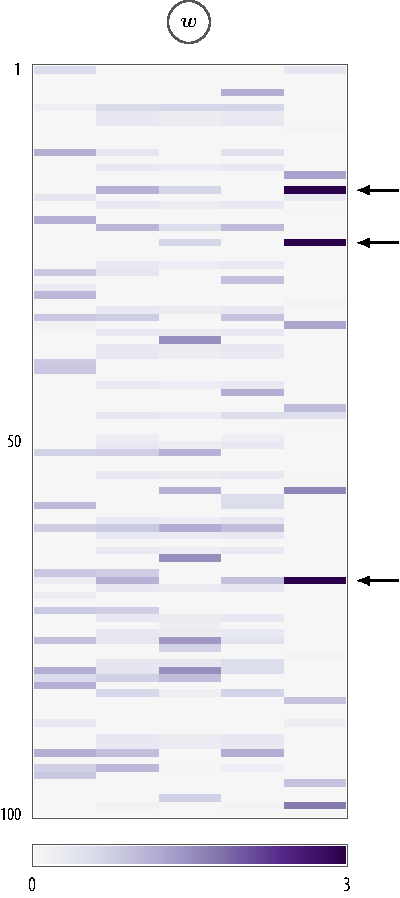
\includegraphics[width=0.6\textwidth]{figures/genes/mat_syn.pdf}\\[1em]
\caption{The $\bw$ matrix of the learned \fldc{} model on a synthetic data set of 100 genes and 500 patients.
The implanted mutually exclusive group of $k = 3$ mutations covers a fraction $\gamma = 0.5$ of the patients, and is distinctly encoded in the last column of the matrix.}
\label{fig:syn_mat}
\end{figure}

To evaluate the ability of our method to recover the true mutually exclusive group, we computed the $F$-measure of the union of the resulting extracted groups compared to the true group.
\figref{fig:syn_single} shows the results across different values of the fraction $\gamma$ of patients covered by the mutually exclusive group, ranging from $0.1$ to $1.0$.
For each value of $\gamma$, we repeat the experiment on $50$ randomly generated data sets.

We show the results of our procedure for two different values of the considered hypothesis testing level $\alpha$, which trades off between false negatives and false positives.
For $\alpha = 0.01$, we have practically perfect recovery when $\gamma \geq 0.4$, but are not able to extract statistically significant groups below $\gamma = 0.3$. 
Using a much higher $\alpha = 0.3$ trades off some false positives to gain statistical power, and exceeds the performance of CoMEt for almost all values of $\gamma$.
Either way, the results show that, in the majority of the cases, the learned \fldc{} model is able to encode the correct group, and propose it for further testing.
We would also like to emphasize at this point that CoMEt takes the size $k = 3$ of the group as input, although it can still output groups of different size; our method, on the other hand, does not use any such information.

\setlength\figureheight{0.7\textwidth}
\setlength\figurewidth{0.95\textwidth}
\begin{figure}[htb]
  \centering
  \begin{tikzpicture}


\colorlet{col1t}{gcol1}
\colorlet{col2t}{gcol2}
\colorlet{col3t}{gcol3}
\colorlet{col4t}{gcol4}
\colorlet{col5t}{gcol5}

\begin{axis}[%
tick label style={font=\sffamily\normalsize},
label style={font=\sffamily\normalsize},
legend style={font=\sffamily\normalsize},
view={0}{90},
width=\figurewidth,
height=\figureheight,
xmin=0, xmax=1.05,
xtick={0, 0.1, 0.2, 0.3, 0.4, 0.5, 0.6, 0.7, 0.8, 0.9, 1.0},
xticklabels={0, 0.1, 0.2, 0.3, 0.4, 0.5, 0.6, 0.7, 0.8, 0.9, 1},
scaled x ticks=false,
xlabel={Fraction of mutated samples},
xlabel shift=0em,
ymin=0, ymax=1.05,
ytick={0, 0.2, 0.4, 0.6, 0.8, 1},
yticklabels={0, 0.2, 0.4, 0.6, 0.8, 1},
ylabel={F-measure},
ylabel shift=0em,
tick label style={/pgf/number format/fixed},
major tick length=2pt,
axis lines*=left,
legend cell align=left,
clip marker paths=true,
legend style={at={(1.0,0.05)},draw=none,row sep=0,anchor=south east},
reverse legend,
every axis plot/.append style={
  mark=*,
  mark size=3,
  line width=2.5pt,
  opacity=1,
}
]

\addplot [
color=col2t,
]
coordinates{
(0.10,0.023)(0.20,0.631)(0.30,0.829)(0.40,0.932)(0.50,0.938)(0.60,0.949)(0.70,0.955)(0.80,0.950)(0.90,0.974)(1.00,0.962)
};
\addlegendentry{CoMEt}

\addplot [
color=col3t,
]
coordinates{
(0.10,0.060)(0.15,0.101)(0.20,0.551)(0.25,0.886)(0.30,0.957)(0.40,0.978)(0.50,0.
978)(0.60,0.957)(0.70,0.994)(0.80,0.973)(0.90,0.973)(1.00,1.000)
};
\addlegendentry{Ours (α = 0.3)}

\addplot [
color=col1t,
]
coordinates{
(0.10,0.000)(0.15,0.000)(0.20,0.000)(0.25,0.000)(0.30,0.800)(0.40,1.000)(0.50,1.
000)(0.60,1.000)(0.70,1.000)(0.80,1.000)(0.90,1.000)(1.00,1.000)
};
\addlegendentry{Ours (α = 0.01)}

\end{axis}
\end{tikzpicture}
  \caption{Results on recovering a single group of $k = 3$ mutually exclusive mutations for different values of the fraction $\gamma$ of patients covered by that group.
  The level $\alpha$ at which we test trades off statistical power at low $\gamma$ for false positives at high $\gamma$.
  }
  \label{fig:syn_single}
\end{figure}

\subsection{Synthetic Data: Multiple Mutually Exlusive Groups}
We move now to the problem of extracting multiple groups of mutually exclusive mutations.
Again, we create synthetic data sets following a procedure outlined by \cite{comet}.
In this case, we start with $20,000$ mutations and $500$ patients, and select $t$ groups of $k$ mutually exclusive mutations.
The number of groups $t$ range from $2$ to $4$, and the mutations per group $k$ from $3$ to $5$.
Each group covers a fraction of patients ranging from $0.4$ to $0.7$, and the mutations of each group cover equal number of patients.
As before, we add $5$ independently mutated genes with high frequencies, as well as random noise.
Finally, we remove genes that are mutated in fewer than $5$ patients, which results in a final ground set of average size $|V| \approx 275$.
To assess the quality of the recovered groups against the true ones, we use the adjusted Rand index \citep{ari}, which is a measure that compares the similarity of two clusterings of a set of elements.
Thus, in our case, an adjusted Rand index of $1$ indicates that the recovered groups are identical to the true ones.

For each combination of $t$ and $k$ we repeated the experiment on $20$ randomly generated data sets.
We ran CoMEt with fixed values of $t = 3$ and $k = 4$, as was done in the original paper \citep{comet}.
\figref{fig:syn_multi} shows the results, in which we see that our method significantly outperforms CoMEt, especially at the lower values of $t$ and $k$.
This showcases the problems encountered by CoMEt (and shared with several other previous methods) when the number and size of the groups to be found is misspecified.
In contrast, we see that our method performs consistently well across all different values of $t$ and $k$, without any knowledge of these parameters.
We also see that, in this case, a higher level $\alpha$ degrades the quality of the final results, because of the frequent occurence of false positives.


\setlength\figureheight{0.65\textwidth}
\setlength\figurewidth{0.95\textwidth}
\begin{figure}[htb]
  \centering
  \begin{tikzpicture}

\colorlet{col1t}{gcol1}
\colorlet{col2t}{gcol2}
\colorlet{col3t}{gcol3}
\colorlet{col4t}{gcol4}
\colorlet{col5t}{gcol5}

\begin{axis}[%
tick label style={font=\sffamily\normalsize},
label style={font=\sffamily\normalsize},
legend style={font=\sffamily\normalsize},
view={0}{90},
width=\figurewidth,
height=\figureheight,
xmin=-0.5, xmax=8.5,
xtick={0, 1, 2, 3, 4, 5, 6, 7, 8},
xticklabels={(2,3), (2,4), (2,5), (3,3), (3,4), (3,5), (4,3), (4,4), (4,5)},
scaled x ticks=false,
xlabel={(t, k)},
xlabel shift=0em,
ymin=0, ymax=1.02,
ytick={0, 0.2, 0.4, 0.6, 0.8, 1},
yticklabels={0, 0.2, 0.4, 0.6, 0.8, 1},
ylabel={Adjusted Rand index},
ylabel shift=0em,
%tick label style={/pgf/number format/fixed},
major tick length=2pt,
axis lines*=left,
legend cell align=left,
clip marker paths=true,
legend style={at={(1.0,0.05)},draw=none,row sep=0,anchor=south east},
ybar,
bar width=12pt
%every axis plot/.append style={
%  mark=none,
%  line width=1.7pt,
%  opacity=0.9,
%}
]

\addplot [
color=col1t,
fill=col1t
]
coordinates{
(0,0.99)(1,0.99)(2,0.99)(3,0.99)(4,0.99)(5,0.99)(6,0.99)(7,0.99)(8,0.99)
};
\addlegendentry{Ours}


\addplot [
color=col2t,
fill=col2t
]
coordinates{
(0,0.53)(1,0.51)(2,0.74)(3,0.68)(4,0.88)(5,0.94)(6,0.8)(7,0.92)(8,0.83)
};
\addlegendentry{CoMEt}


\end{axis}
\end{tikzpicture}
  \caption{Results on recovering $t$ groups of $k$ mutually exclusive mutations.
Our method performs consistently well across all different $t$ and $k$, while CoMEt performs poorly when $t$ and $k$ are misspecified.
  }
  \label{fig:syn_multi}
\end{figure}

\subsection{Real Cancer Data}
We analyzed two real cancer data sets from TCGA, the first pertaining to acute myeloid leukemia \citep{tcga_aml}, and the second to breast cancer \citep{tcga_brca}.
For both data sets, we used the preprocessed versions by \cite{comet} available on GitHub\footnote{\url{https://github.com/raphael-group/comet}}.

\paragraph{Acute myeloid leukemia (AML).}
The data set consists of 51 mutations and 200 patients.
The learned \fldc{} model ($L = 10$) is shown in \figref{fig:mat_aml}.
We have annotated on the two matrices the discovered mutually exclusive and co-occurring groups that have (uncorrected) $p$-values $\leq 0.01$ for both $p_{\mathrm{gf}}$ and $p_{\mathrm{ova}}$.
(We have also decided to include group $R_2$, even though its $p_{\mathrm{ova}}$ is barely above $0.01$.)

\figsref{fig:rep_aml_1} and \ref{fig:rep_aml_2} illustrate in detail each of the mutually exclusive groups $R_1$--$R_8$ by showing the corresponding permuted data rows, as well as the computed $p$-values for each group.
\figref{fig:graph_aml} summarizes these eight groups into a graphical structure.
Each node represents a mutation, with darker nodes corresponding to higher marginal frequency in the data set.
The mutually exclusive groups are shown shaded, with darker groups corresponding to lower $p_{\mathrm{ova}}$.
\figref{fig:att_aml} shows the five discovered groups $A_1$--$A_5$ of co-occurring mutations.

\begin{figure}[htbp]
\centering
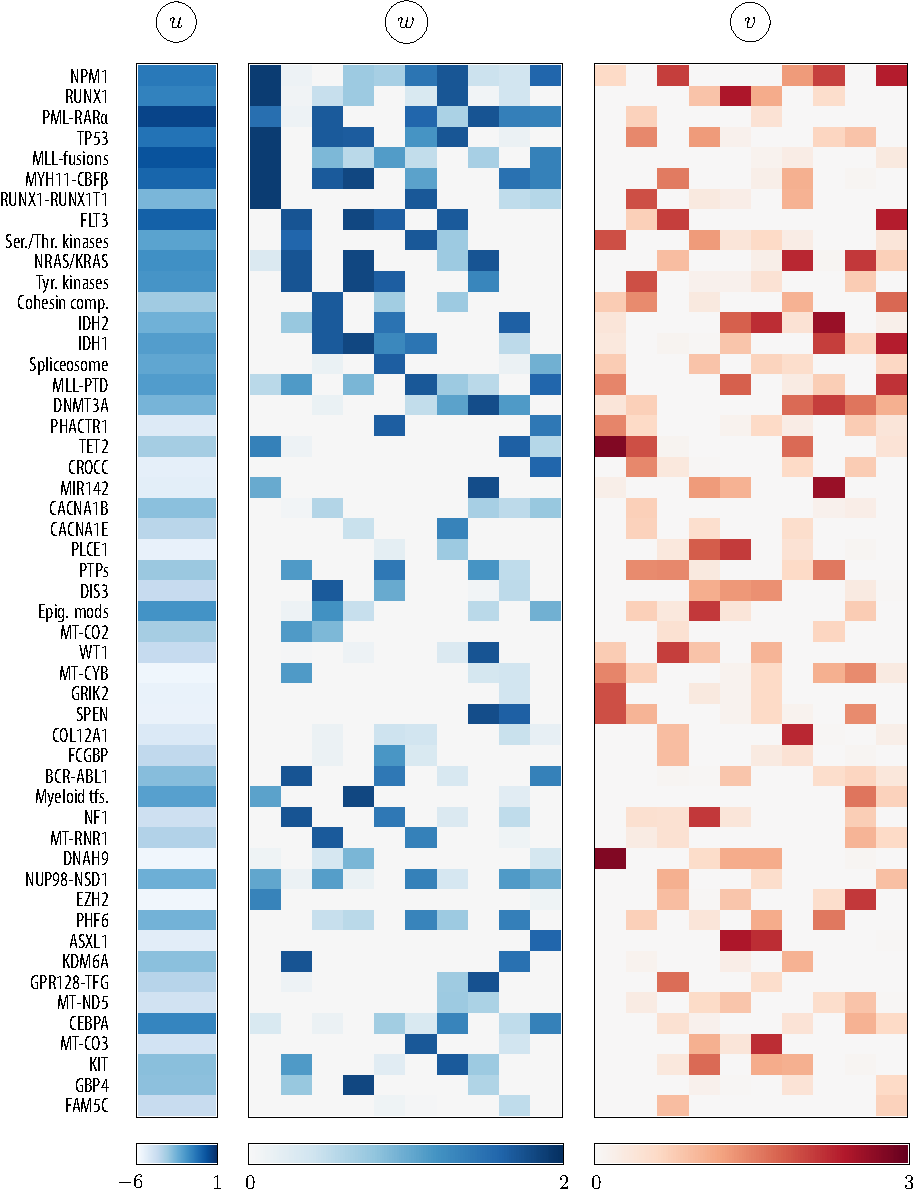
\includegraphics[width=\textwidth]{figures/genes/mat_aml.pdf}\\[1em]
\caption{The learned utility ($\bu$), repulsive ($\bw$), and attractive ($\bv$) matrices of the \fldc{} model ($L = 10$) on the TCGA AML data set.
We have permuted the rows and columns to bring the discovered groups towards the upper left of the matrices.
Groups $R_1$--$R_8$ are mutually exclusive, while groups $A_1$--$A_5$ are co-occurring.
}
\label{fig:mat_aml}
\end{figure}

\begin{figure}[htbp]
\centering
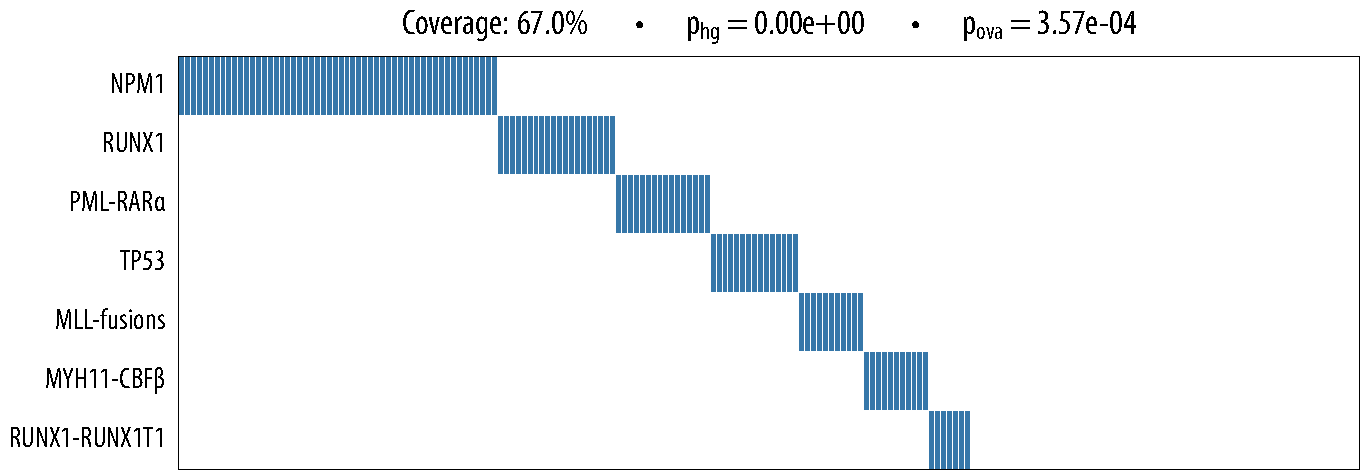
\includegraphics[width=\textwidth]{figures/genes/aml_1.pdf}\\[2em]
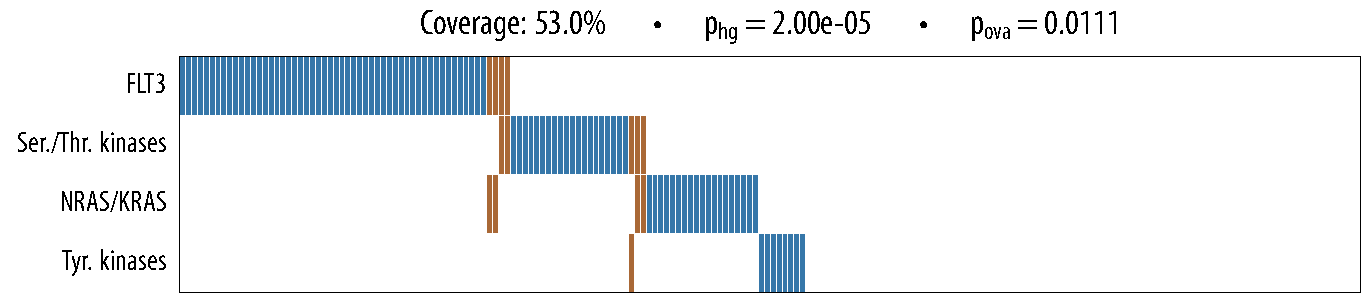
\includegraphics[width=\textwidth]{figures/genes/aml_2.pdf}\\[2em]
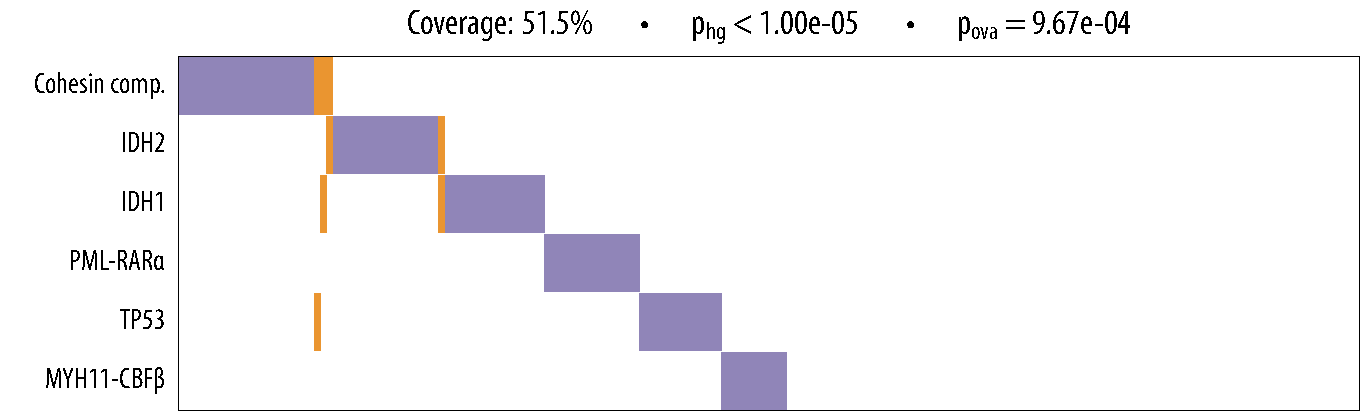
\includegraphics[width=\textwidth]{figures/genes/aml_3.pdf}\\[2em]
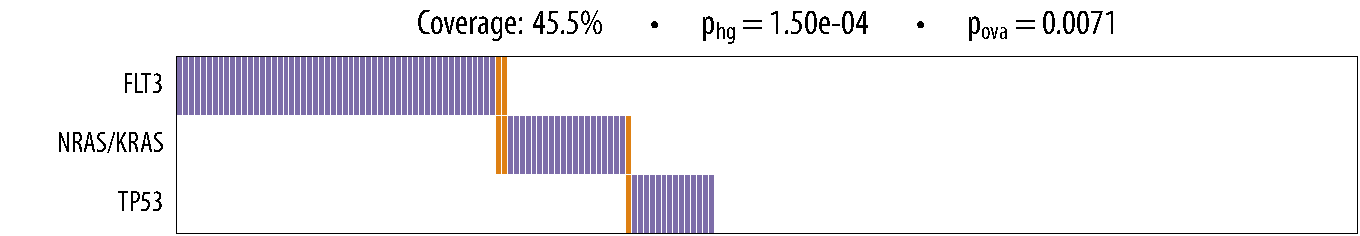
\includegraphics[width=\textwidth]{figures/genes/aml_4.pdf}\\[2em]
\caption{The first four mutually exclusive groups extracted from the TCGA AML data set.
Each row corresponds to a mutation, and each column to a patient.
The highlighted entries represent co-occurring mutations.}
\label{fig:rep_aml_1}
\end{figure}

\begin{figure}[htbp]
\centering
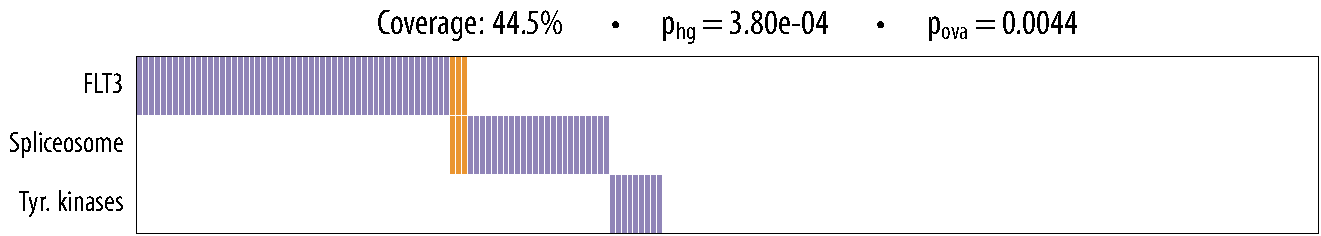
\includegraphics[width=\textwidth]{figures/genes/aml_5.pdf}\\[2em]
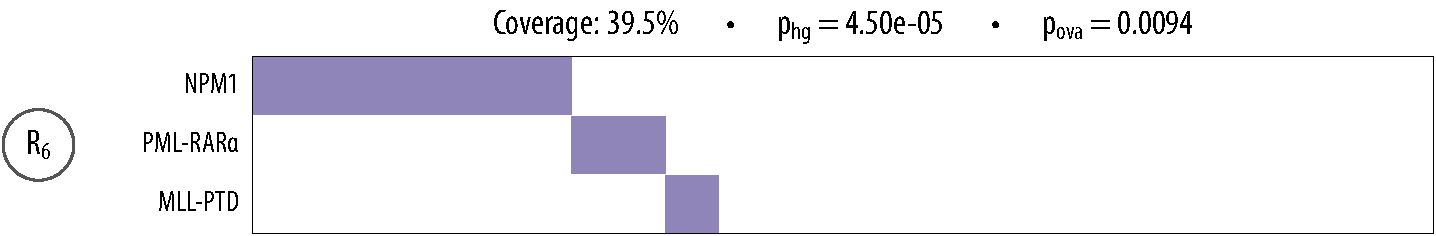
\includegraphics[width=\textwidth]{figures/genes/aml_6.pdf}\\[2em]
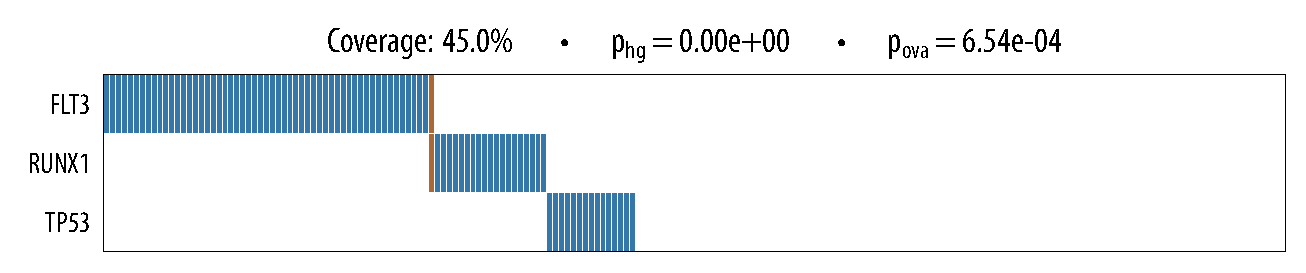
\includegraphics[width=\textwidth]{figures/genes/aml_7.pdf}\\[2em]
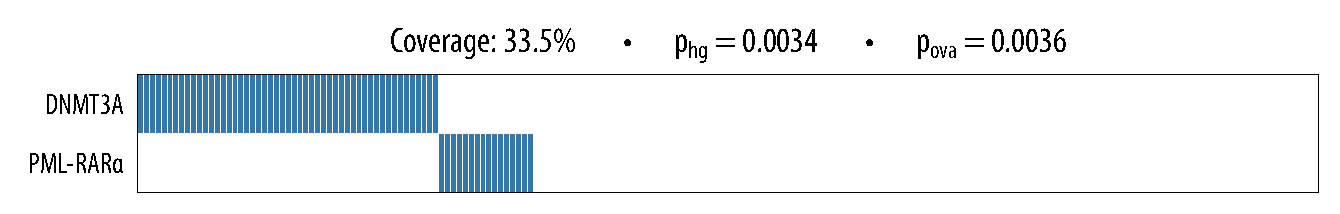
\includegraphics[width=\textwidth]{figures/genes/aml_8.pdf}\\[2em]
\caption{The next four mutually exclusive groups extracted from the TCGA AML data set.
Each row corresponds to a mutation, and each column to a patient.
The highlighted entries represent co-occurring mutations.}
\end{figure}

\begin{figure}[htbp]
\centering
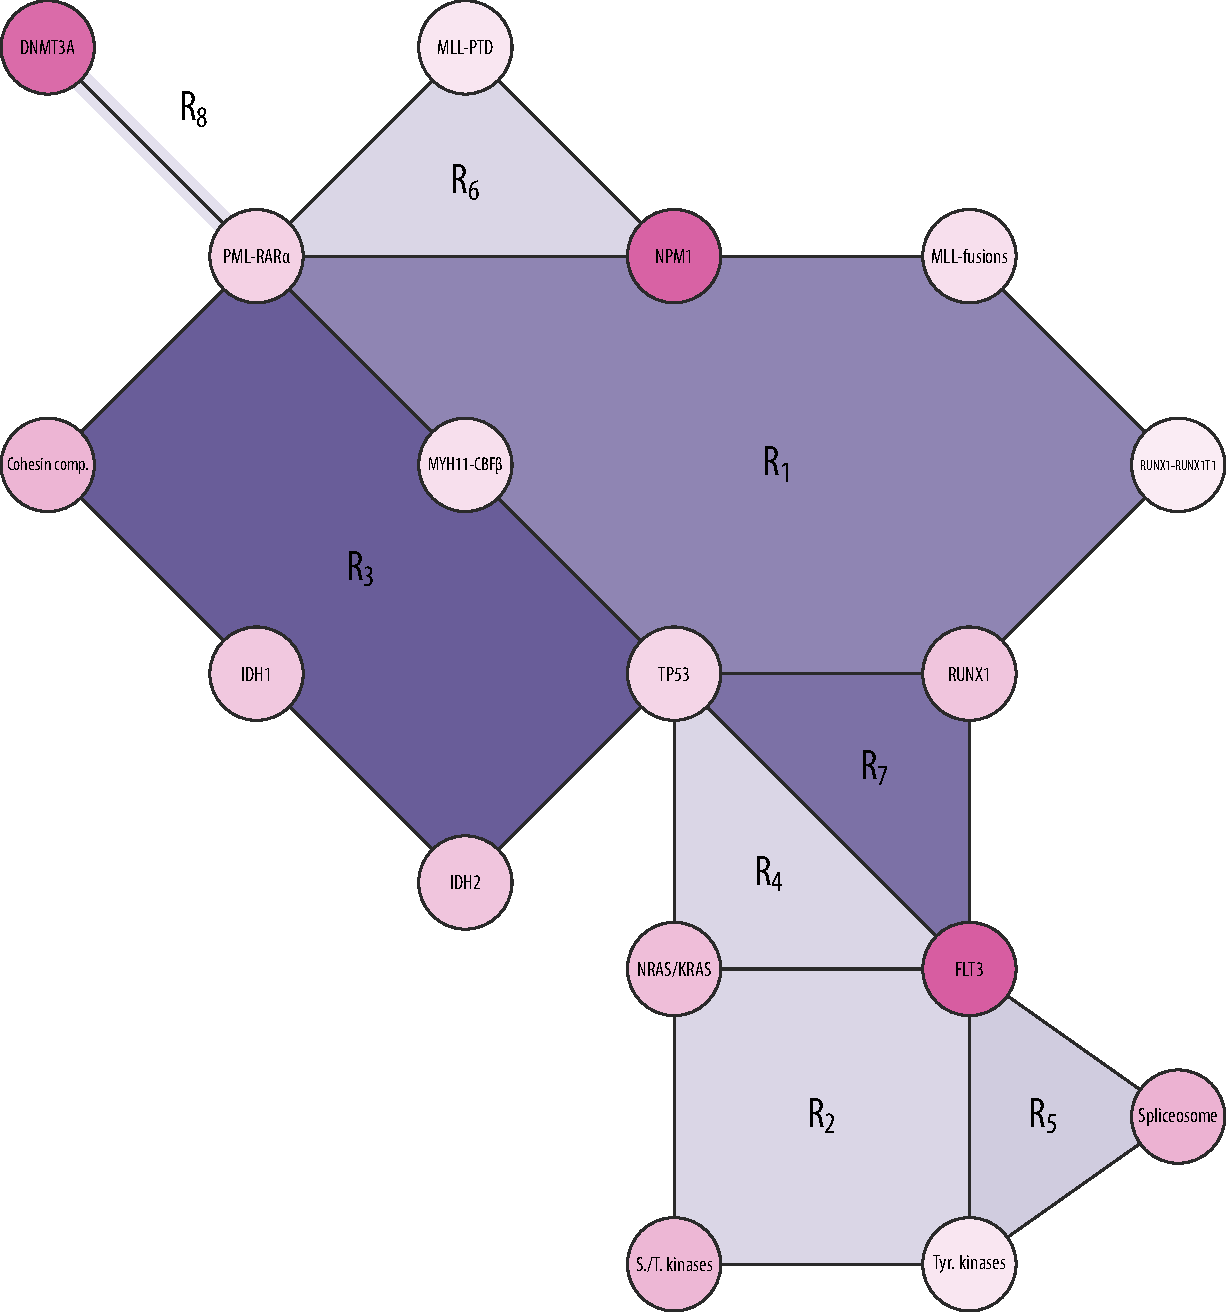
\includegraphics[width=\textwidth]{figures/genes/graph_aml.pdf}\\[2em]
\caption{A graphical representation of the eight discovered mutually exclusive groups in the TCGA AML data set.
Darker nodes correspond to more frequent mutations, and darker shaded polygons correspond to more significant (that is, lower $p_{\mathrm{ova}}$) groups.}
\label{fig:graph_aml}
\end{figure}

\begin{figure}[htbp]
\centering
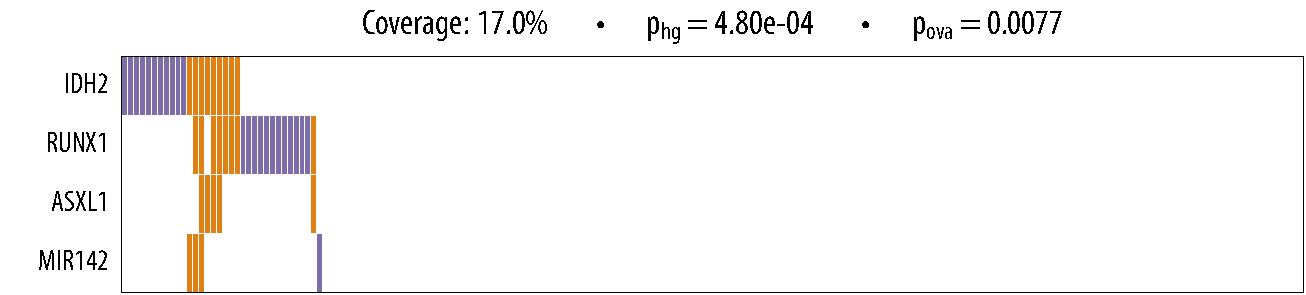
\includegraphics[width=\textwidth]{figures/genes/aml_2_a.pdf}\\[2em]
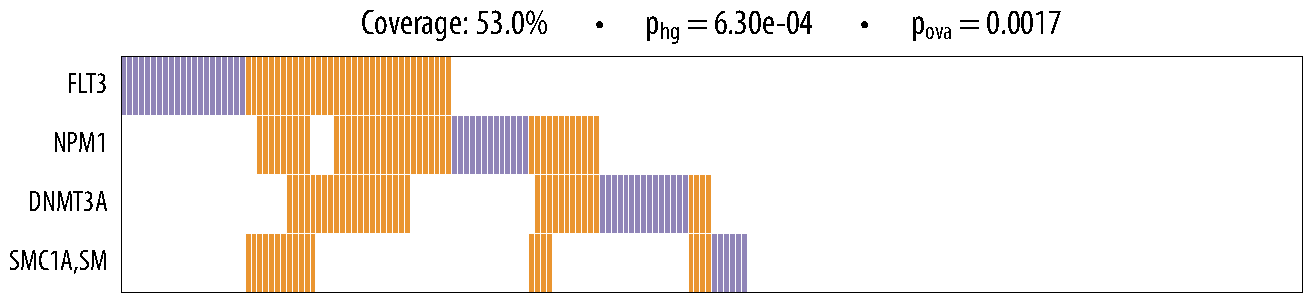
\includegraphics[width=\textwidth]{figures/genes/aml_1_a.pdf}\\[2em]
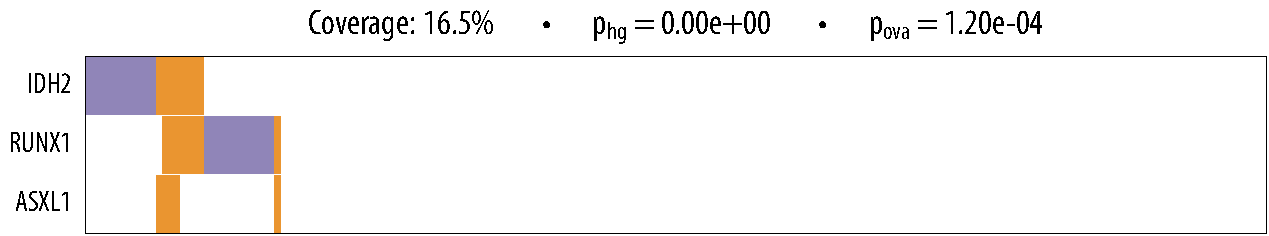
\includegraphics[width=\textwidth]{figures/genes/aml_3_a.pdf}\\[2em]
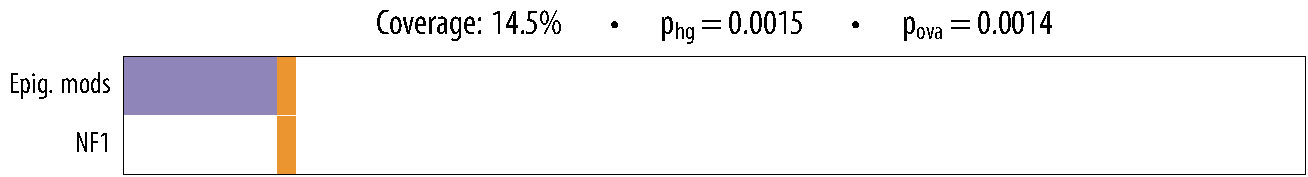
\includegraphics[width=\textwidth]{figures/genes/aml_5_a.pdf}\\[2em]
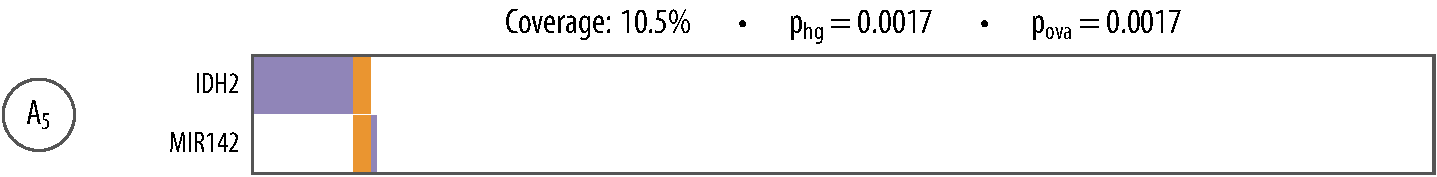
\includegraphics[width=\textwidth]{figures/genes/aml_4_a.pdf}\\[2em]
\caption{The five co-occurring groups extracted from the TCGA AML data set.
Each row corresponds to a mutation, and each column to a patient.
The highlighted entries represent co-occurring mutations.}
\label{fig:att_aml}
\end{figure}

It is notable that CoMEt detects groups $R_1$ (without the last mutation, \textsf{RUNX1-RUNX1T1}) and $R_2$, but fails to detect any of the other six groups, even though almost all of them have particularly low $p_{\mathrm{gf}}$.
We suspect that this is caused by the combination of CoMEt using as input a fixed number of groups and sizes thereof, as well as the fact that their searching procedure based on sampling works on a particularly slow-mixing landscape.
As an example, although they are searching for a group of size $6$, they never discover our group $R_3$, because their sampler presumably gets stuck on group $R_1$, which has a few orders of magnitude lower $p_{\mathrm{gf}}$ compared to $R_3$.
On the other hand, CoMEt detects two other groups (see \figref{fig:comet_aml}), which have $p_{\mathrm{ova}}$ significantly above our cutoff, and furthermore, also have $p_{\mathrm{gf}}$ significantly higher than all our discovered groups, except for $R_8$.
For a comparison of the discovered mutation interactions, we also refer to \citep[Figure S8]{tcga_aml}, which confirms many of our findings, although it only illustrates pairwise interactions.

\paragraph{Breast cancer (BRCA).}
The data set consists of 375 mutations and 507 patients.
We show the resulting learned \fldc{} model ($L = 15$) in \figref{fig:mat_brca}, the extracted mutually exclusive groups $R_1$--$R_{11}$ in \figsref{fig:rep_brca_1} and \ref{fig:rep_brca_2}, and a graphical summarization of all these groups in \figref{fig:graph_brca}.
In \figref{fig:att_brca_1} we show the six extracted co-ocurring groups with the highest coverage; groups $A_7$--$A_{14}$ can be found in \figref{fig:att_brca_2} in the appendix.

The CoMEt results on BRCA take into account additional information about the classification of each patient into four different subtypes of breast cancer.
While this means that we cannot directly compare our results to theirs, we still recover some of their findings (e.g., the first three mutations in $R_1$), but also extract significant groups that were not found by CoMEt, even when constrained to a specific subtype (e.g., $R_3$ for the ``Luminal-A'' subtype).
Furthermore, we observe that the co-occurring groups $A_1$--$A_6$ are particularly significant, with $p$-values of order $10^{-5}$ or less.

\begin{figure}[htbp]
\centering
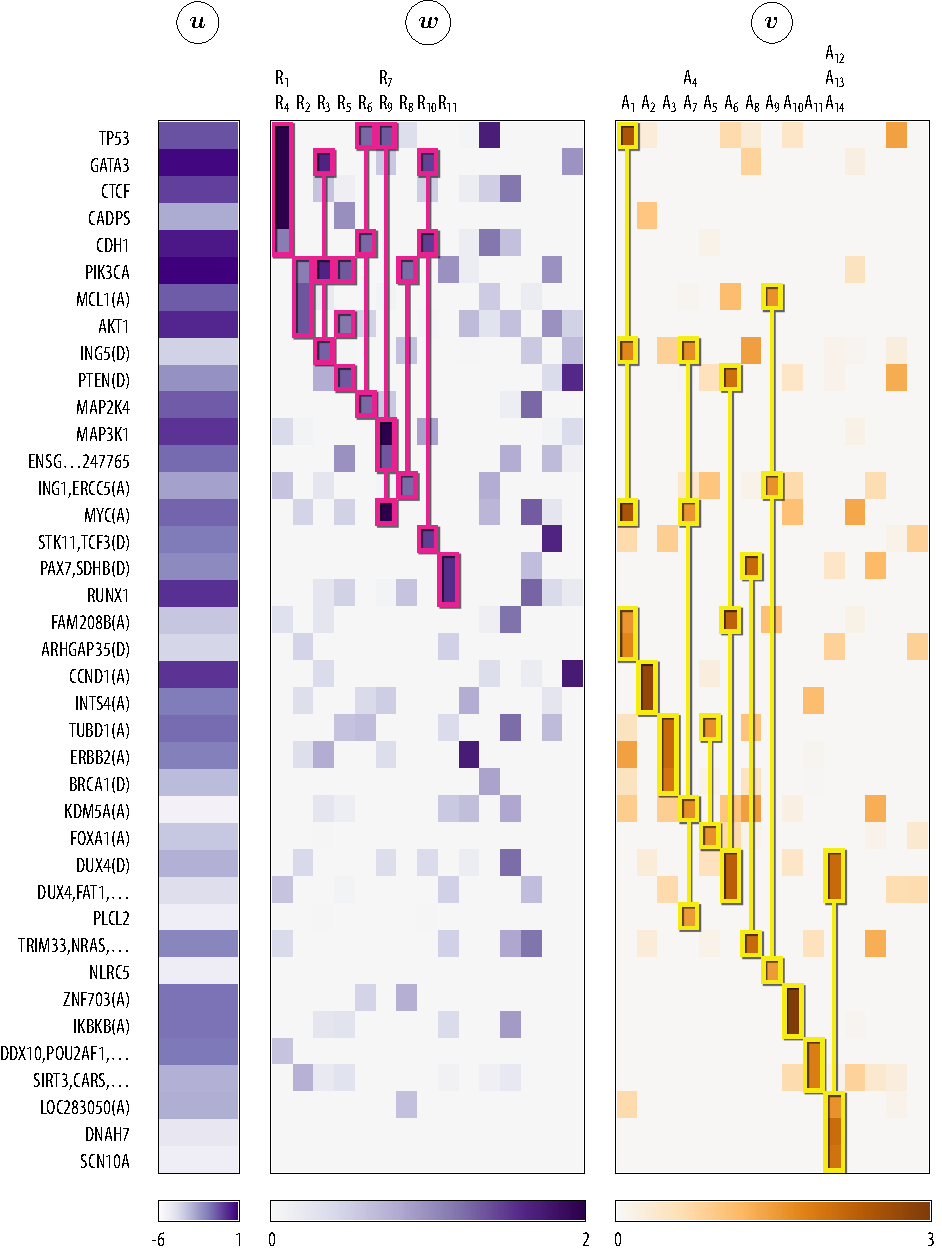
\includegraphics[width=\textwidth]{figures/genes/mat_brca.pdf}\\[2em]
\caption{The learned utility ($\bu$), repulsive ($\bw$), and attractive ($\bv$) matrices of the \fldc{} model ($L = 15$) on the TCGA BRCA data set.
For illustration purposes, we only show the submatrices corresponding to the $39$ mutations that participate in the extracted groups.
We have also permuted the rows and columns to bring these groups towards the upper left of the matrices.
Groups $R_1$--$R_{11}$ are mutually exclusive, while groups $A_1$--$A_{14}$ are co-occurring.
}
\label{fig:mat_brca}
\end{figure}

\begin{figure}[htbp]
\centering
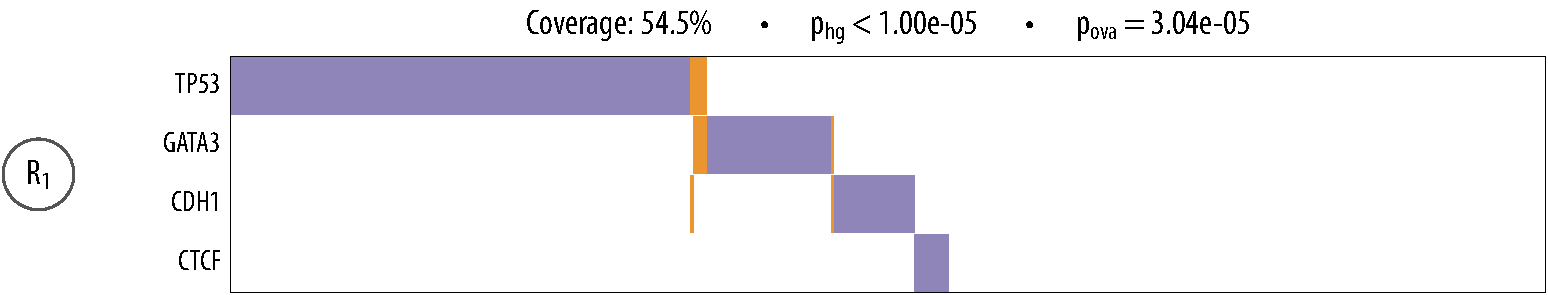
\includegraphics[width=\textwidth]{figures/genes/brca_1.pdf}\\[2em]
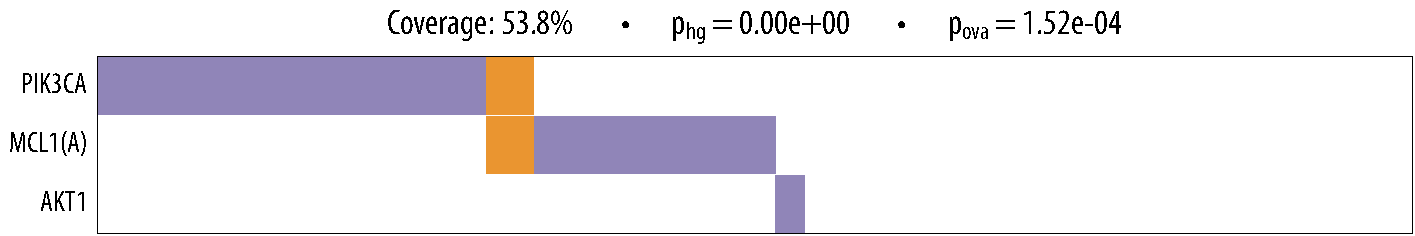
\includegraphics[width=\textwidth]{figures/genes/brca_6.pdf}\\[2em]
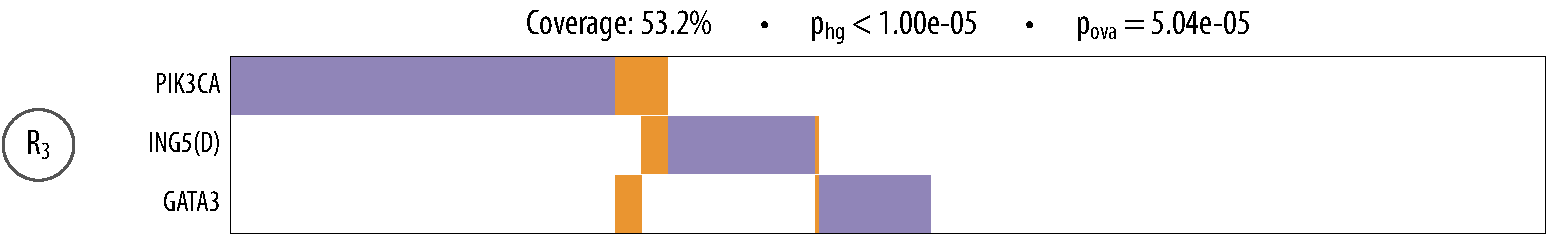
\includegraphics[width=\textwidth]{figures/genes/brca_8.pdf}\\[2em]
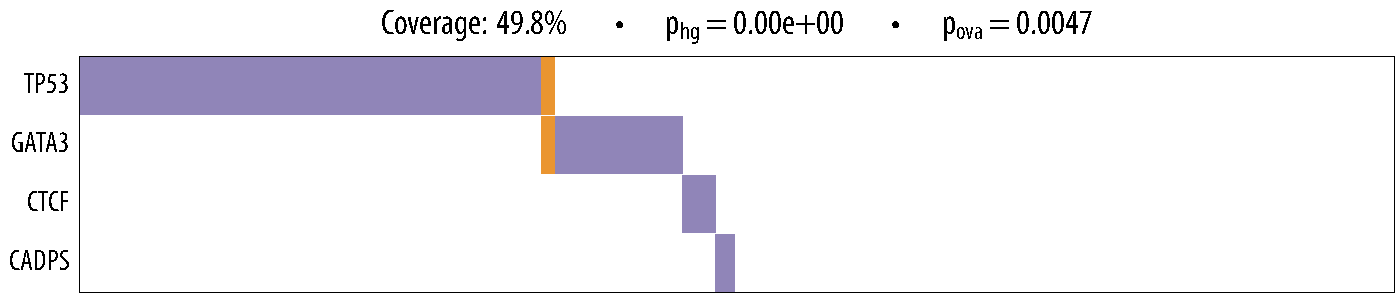
\includegraphics[width=\textwidth]{figures/genes/brca_2.pdf}\\[2em]
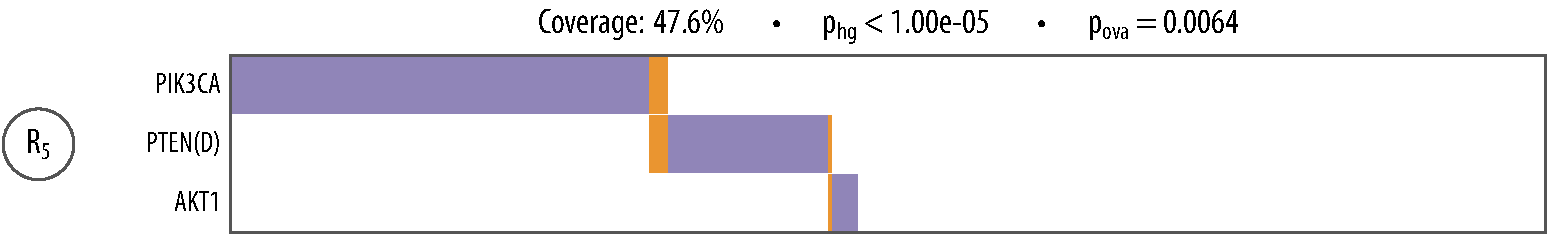
\includegraphics[width=\textwidth]{figures/genes/brca_5.pdf}\\[2em]
\caption{The first five mutually exclusive groups extracted from the TCGA BRCA data set.
Each row corresponds to a mutation, and each column to a patient.
The highlighted entries represent co-occurring mutations.}
\label{fig:rep_brca_1}
\end{figure}

\begin{figure}[htbp]
\centering
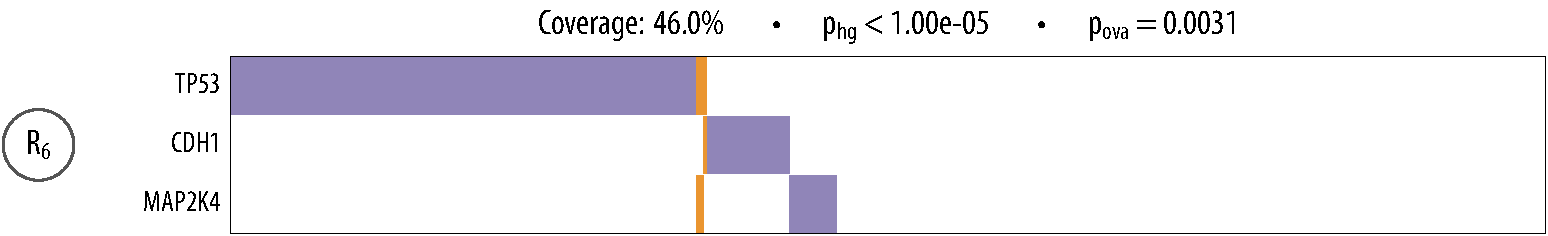
\includegraphics[width=\textwidth]{figures/genes/brca_4.pdf}\\[2em]
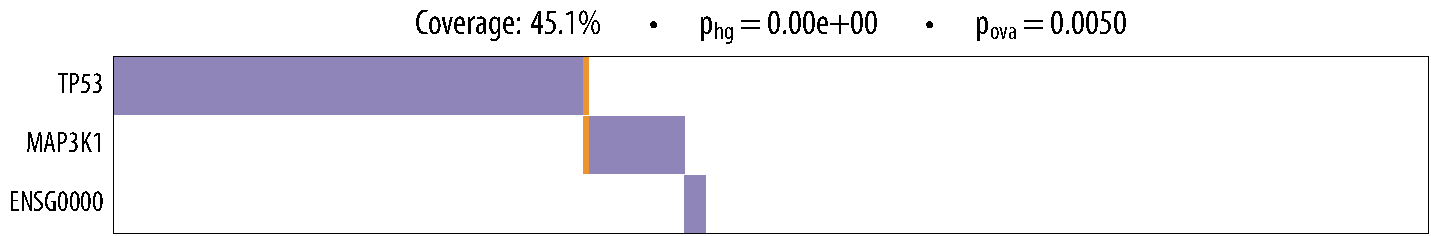
\includegraphics[width=\textwidth]{figures/genes/brca_3.pdf}\\[2em]
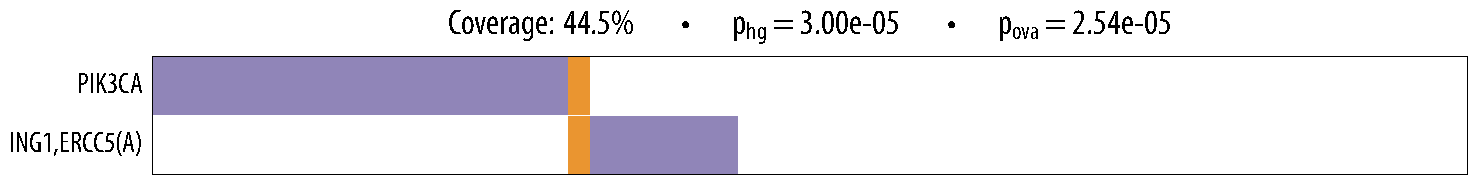
\includegraphics[width=\textwidth]{figures/genes/brca_11.pdf}\\[2em]
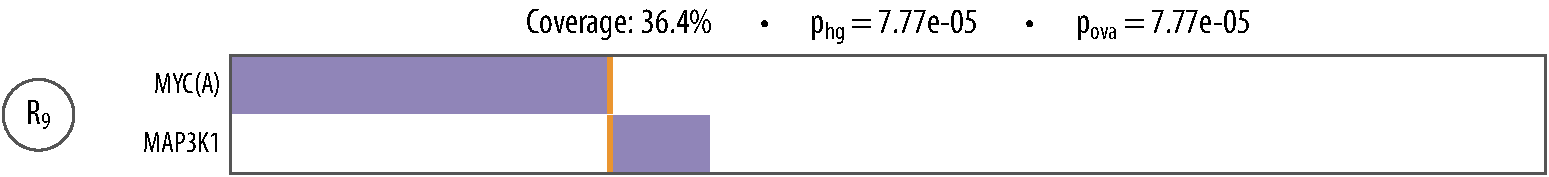
\includegraphics[width=\textwidth]{figures/genes/brca_10.pdf}\\[2em]
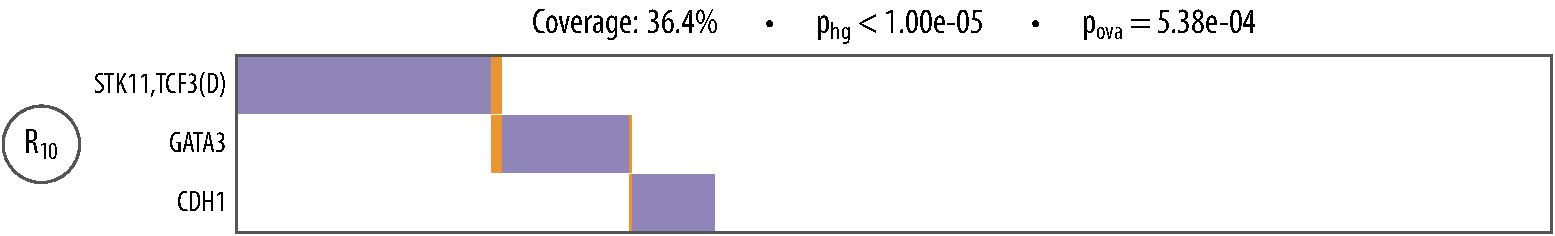
\includegraphics[width=\textwidth]{figures/genes/brca_7.pdf}\\[2em]
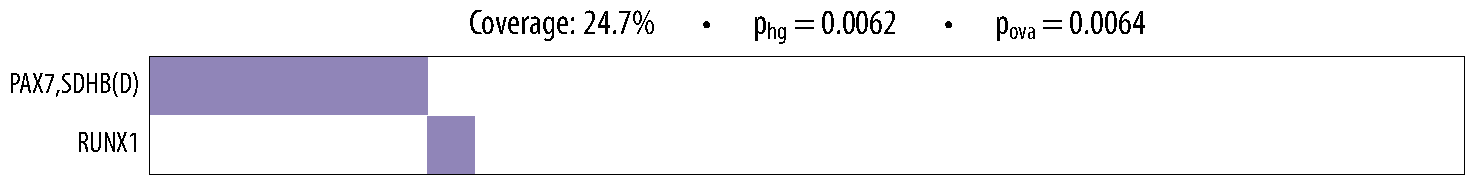
\includegraphics[width=\textwidth]{figures/genes/brca_9.pdf}\\[2em]
\caption{The next six mutually exclusive groups extracted from the TCGA BRCA data set.
Each row corresponds to a mutation, and each column to a patient.
The highlighted entries represent co-occurring mutations.}
\label{fig:rep_brca_2}
\end{figure}

\begin{figure}[htbp]
\centering
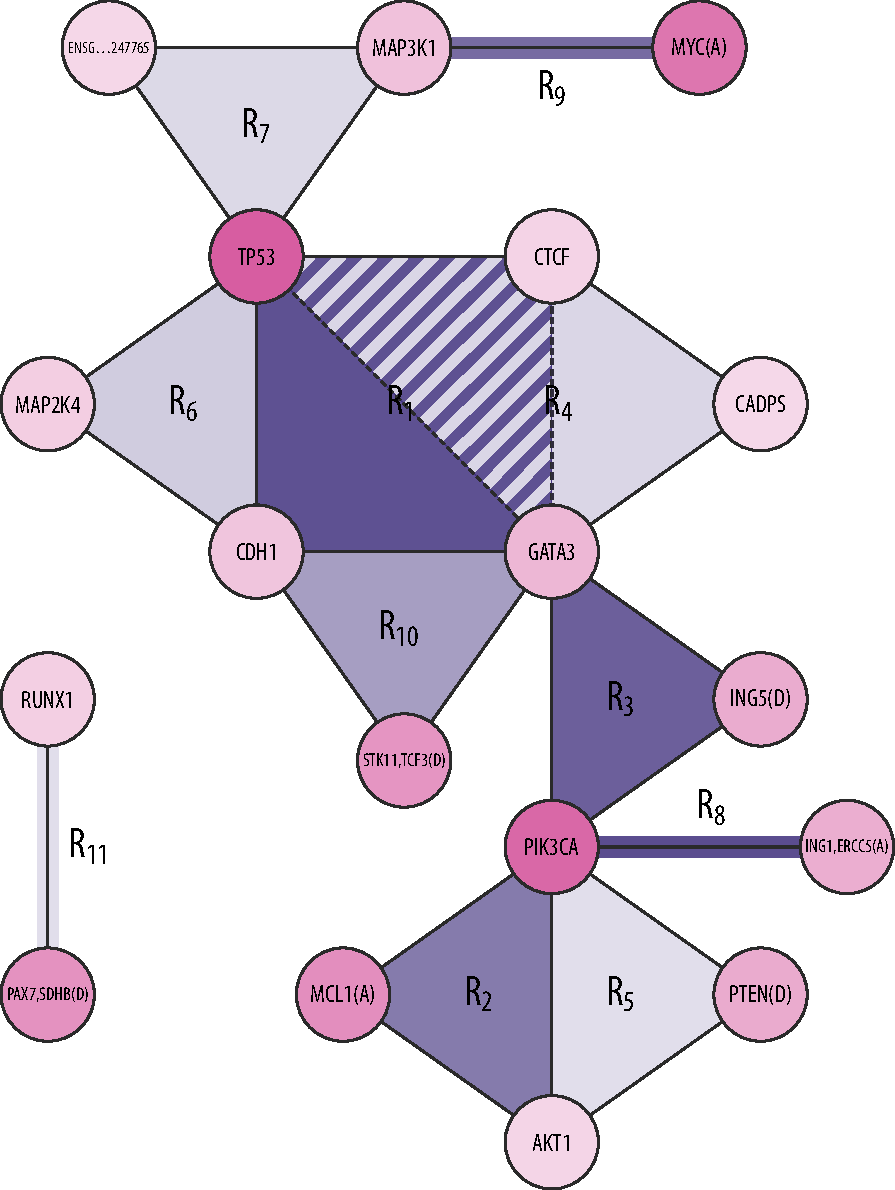
\includegraphics[width=\textwidth]{figures/genes/graph_brca.pdf}\\[2em]
\caption{A graphical representation of the $11$ discovered mutually exclusive groups in the TCGA BRCA data set.
Darker nodes correspond to more frequent mutations, and darker shaded polygons correspond to more significant (that is, lower $p_{\mathrm{ova}}$) groups.}
\label{fig:graph_brca}
\end{figure}

\begin{figure}[htbp]
\centering
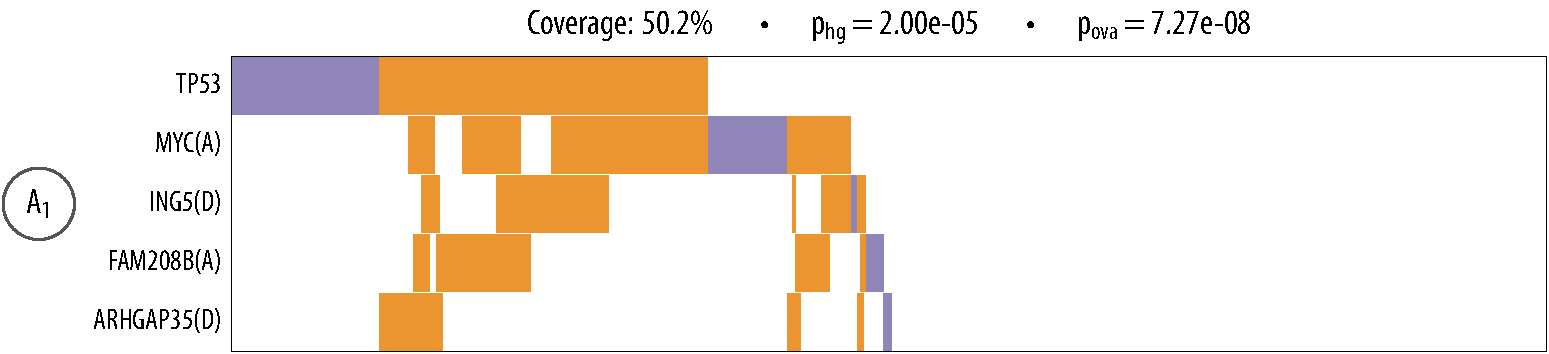
\includegraphics[width=\textwidth]{figures/genes/brca_1_a.pdf}\\[2em]
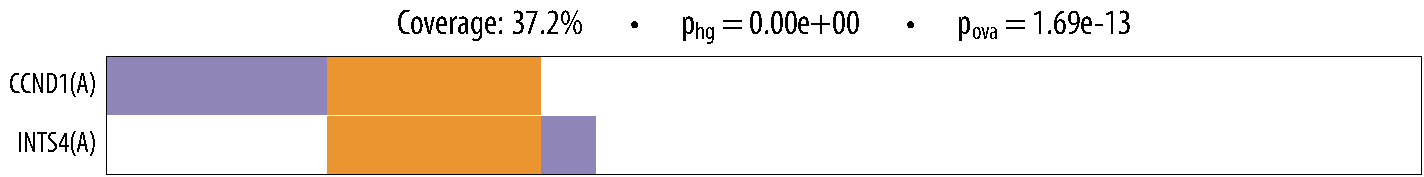
\includegraphics[width=\textwidth]{figures/genes/brca_11_a.pdf}\\[2em]
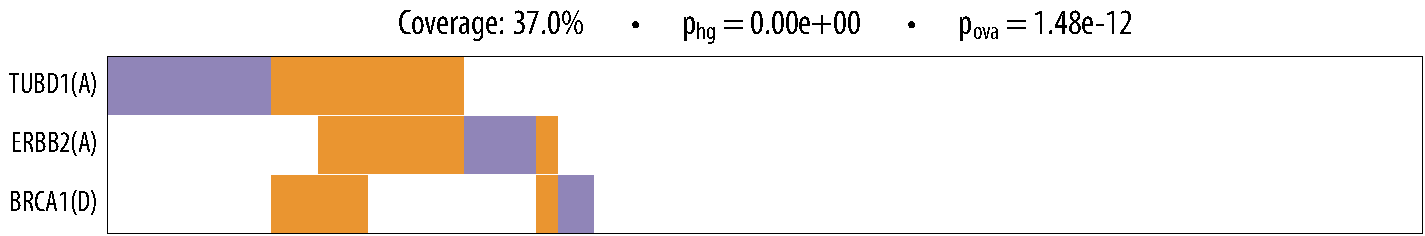
\includegraphics[width=\textwidth]{figures/genes/brca_7_a.pdf}\\[2em]
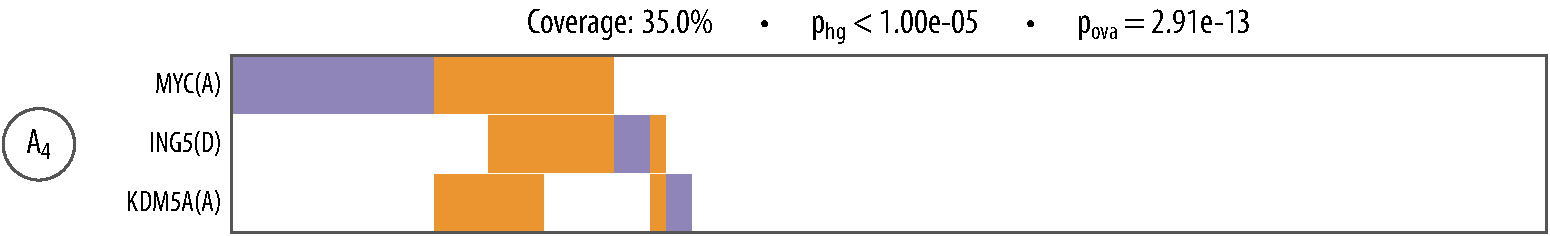
\includegraphics[width=\textwidth]{figures/genes/brca_8_a.pdf}\\[2em]
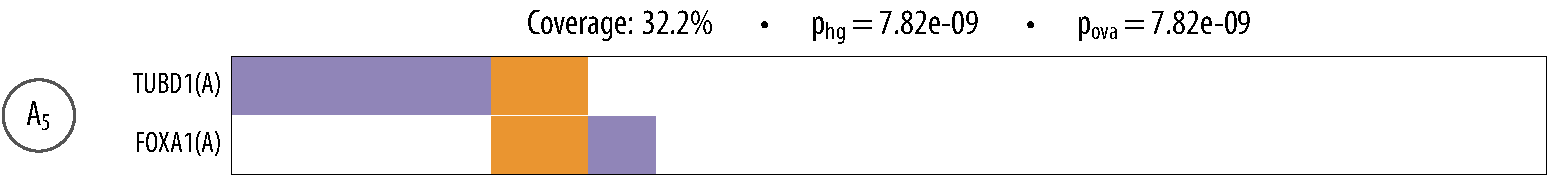
\includegraphics[width=\textwidth]{figures/genes/brca_14_a.pdf}\\[2em]
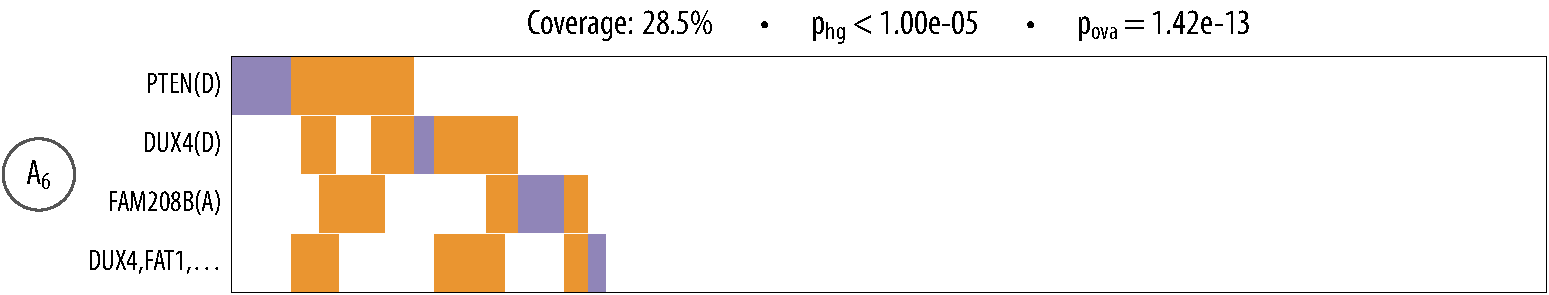
\includegraphics[width=\textwidth]{figures/genes/brca_4_a.pdf}\\[2em]
\caption{The first six co-occurring groups extracted from the TCGA BRCA data set.
Each row corresponds to a mutation, and each column to a patient.
The highlighted entries represent co-occurring mutations.}
\label{fig:att_brca_1}
\end{figure}

\section{Conclusion}
In this chapter, we have seen how sampling can be effectively used to obtain estimates of the gradient of a probabilistic submodular model with respect to its parameters.
It, thus, facilitates applying an approximate maximum likelihood maximization procedure to learn such models from data.
We have applied this learning procedure to the problem of modeling interactions of genetic mutations in cancer patients, with the particular goal of discovering groups of mutually exlusive and co-occurring mutations.
We have shown that our method often outperforms the state of the art for this task by naturally capturing these higher-order interactions without the need to prespecify the number or size of groups to be found.